\documentclass[msc]{ppgccufmg}

\usepackage[brazil]{babel}     
\usepackage[utf8]{inputenc}
\usepackage[T1]{fontenc}
\usepackage{type1ec}
\usepackage{graphicx}
\usepackage{multirow}
\usepackage{rotating}
\usepackage{subfig}
\usepackage{amssymb}
\usepackage{color}
\usepackage{epsfig}
\usepackage[a4paper,
  portuguese,
  bookmarks=true,
  bookmarksnumbered=true,
  linktocpage,
  colorlinks,
  citecolor=black,
  urlcolor=black,
  linkcolor=black,
  filecolor=black,
  ]{hyperref}
\usepackage{algorithm}
%\usepackage{algorithmic}
\usepackage[noend]{algpseudocode}
% \usepackage[Algoritmo]{algorithm}
% \usepackage[noend]{algpseudocode}
\usepackage{ae}
\usepackage[square]{natbib}
\usepackage{amsmath}
\usepackage{amsthm}

\bibpunct{[}{]}{;}{a}{,}{,}
\usepackage{url}

\usepackage{natbib}
\begin{document}

% O comando a seguir, \ppgccufmg, prove todas as informações relevantes para a
% classe ppgccufmg. Por favor, consulte a documentação para a descrição de
% cada chave.

\ppgccufmg{
  title={TITULO DO MEU TRABALHO},
  authorrev={Palotti, João Rafael de Moura},
  cutter={D1234p},
  cdu={519.6*82.10},
  university={Universidade Federal de Minas Gerais},
  course={Ciência da Computação},
  address={Belo Horizonte},
  date={2010-10},
  keywords={Classificação, Mineração de Dados, Computação Evolucionária, Programação Genética},
  advisor={Gisele Lobo Pappa},
  abstract={Resumo}{resumo},
  abstract=[english]{Abstract}{abstract},
%  ack={agradecimentos},
  epigraphtext={Veni, Vidi, Vici}{Julius Caesar},
}

%-------------------------------------------------------------
\chapter{Introdução}
\label{cap::introducao}
\chapter{Introdução}
\label{cap::introducao}


É inegável que vivemos em uma época na qual temos uma capacidade nunca antes vista de gerar informação.
A possibilidade de interagir com outros pessoas através da \textit{Web} usando redes sociais com milhões de usuários (\cite{Thom11}), criar \textit{blogs} com textos, vídeos e músicas (\cite{Baxter10}), extrair informações a respeito de todos os genes que formam organismos complexos como os nossos (\cite{Williams01}), obter informações sobre as condições climáticas de um região com sensores que captam centenas de variáveis simultaneamente (\cite{Rotach09}), são alguns entre os diversos exemplos de nossa capacidade de produzir informação.
Entretanto, proporcionalmente ao aumento da disponibilidade desses dados, vemos também o aumento da dificuldade em analisar, compreender e classificar essas informações.

Organizar e recuperar grandes quantidades de informação tornaram-se tarefas de extrema importância, principalmente nas áreas de Mineração de Dados e Recuperação de Informação, responsáveis por estudar uma maneira de lidar com essa explosão de dados. Dentre as diversas tarefas estudadas por essas duas áreas destacamos a \textbf{Classificação Automática} de dados. 

Nesta dissertação, tratamos o problema de classificar automaticamente a informação disponível. 
Substituir humanos por máquinas na tarefa de classificação não somente é útil, como necessário. 
Seria entediante e, muito provavelmente, impraticável para um humano classificar uma grande quantidade de dados.

De maneira simplificada, classificar consiste em estipular a qual classe, dentre as disponíveis, um certo exemplo 
pertence, partindo da premissa que dois exemplos estão em uma mesma classe se eles possuem um valor semântico próximo. 
Em geral, temos um conjunto de exemplos conhecidos, dos quais sabemos a que classe cada exemplo pertence, e um conjunto de exemplos com classe desconhecida, para os quais queremos prever a classe. O primeiro conjunto é chamado de treinamento, e o segundo de teste. 

De forma geral, humanos e computadores conseguem construir um modelo de classificação a partir dos exemplos presentes no treinamento. 
Analisando os atributos, as semelhanças e as diferenças que fazem com que um exemplo pertença a uma classe ou a outra, um classificador, humano ou não, pode aprender, através de observações, uma maneira de classificar os exemplos de teste.
Porém, existe uma diferença entre um humano e um algoritmo de classificação automática tradicional. 
Um humano é capaz de ponderar se um dado exemplo do conjunto de treinamento pode contribuir mais ou menos para a geração de um modelo de classificação.
Isso significa que, em uma situação em que temos um exemplo difícil de classificar, dada a sua semelhança com exemplos existentes em mais de uma classe, o classificador humano pode escolher dar maior credibilidade para alguns exemplos de treino, confiando que determinados exemplos podem se assemelhar mais ao teste.

O estudo da capacidade humana de atribuir diferentes valores de credibilidade para as informações apresentadas impulsionou as pesquisas na área de credibilidade. 
Em geral, os pesquisadores estudam como alguns fatores (também chamados de dimensões) afetam na percepção humana de credibilidade.
Eles tentam obter respostas para questões como: o que pode levar um humano a dizer que a informação A tem maior credibilidade que a informação B?
Entretanto, o conceito de credibilidade nunca foi empregado do ponto de vista de um classificador automático. Dado que algumas informações são mais pertinentes que outras, buscamos nesse trabalho avaliar como explorar esse conhecimento para melhorar algoritmos de classificação automática.

Portanto, buscamos uma maneira de criar modelos de classificação que levem em conta o fato que os exemplos de treinamento não são todos igualmente significativos, assim como um humano faz.
Logo, procuramos avaliar de forma automática a credibilidade dos exemplos de treinamento a fim de que aqueles exemplos com maior credibilidade possam ter maior relevância para classificar um exemplo de teste desconhecido.

Um fato importante observado na literatura é que a credibilidade não é uma propriedade fixa de um exemplo, podendo ser diferente dependendo de quem a estipula. Dessa forma, para se obter uma medida menos subjetiva, é necessário definir bem os fatores que influenciam na credibilidade de um exemplo. Neste trabalho, abordamos dois fatores que julgamos ser cruciais: (i) os atributos que compõem um exemplo e (ii) os relacionamentos mantidos entre os exemplos de treino e teste.

Para explorar a credibilidade de um exemplo usando os seus atributos, procuramos medir diretamente a relevância dos atributos na classificação. Assim, utilizamos métricas conhecidas de seleção de atributos para modelarmos a relação atributo-classe. Essa modelagem tem por objetivo prover indícios da separação entre as classes, capturando assim, a importância e a confiança de um exemplo de treinamento para uma classe.

Podemos imaginar diversos exemplos práticos na tarefa de Classificação Automática de Documentos (\textsc{CAD}), que é especialização da classificação automática voltada para definir classes a documentos. Cada documento é composto por um conjunto de termos que são os seus atributos. Nesse caso, se um portal de notícias decidisse incorporar a credibilidade de atributos em seu classificador, provavelmente, ao avaliar a credibilidade baseada nos atributos, veríamos que o termo ``Metallica'' teria maior credibilidade que o termo ``Anthrax'' para prevermos que um documento é da classe Música. Isso acontece porque ``Metallica'' tradicionalmente se refere a uma banda de metal e seria um termo usado para definirmos exclusivamente a classe ``Música'', enquanto ``Anthrax'' além de ser o nome de uma banda, também é uma doença bacteriana. Logo, ele não é tão confiável para distinguir entre ``Música'' e ``Saúde''.
Concluindo, analisando esses termos isoladamente, documentos de treino contendo o termo ``Metallica'' devem ter uma credibilidade maior que documentos contendo o termo ``Anthrax'' do ponto de vista de um classificador que pretende calcular se um documento de teste pertence a classe ``Música''.

Por sua vez, para explorar a credibilidade de um exemplo usando os seus relacionamentos, temos que primeiro definir quais são esses relacionamentos, se eles existirem. 
Vários relacionamentos podem ser definidos dependendo do contexto que estamos abordando. Por exemplo, pessoas mantêm relacionamentos de amizade ou parentesco, livros e músicas têm relacionamentos de autorias, um país se relaciona com outro definindo estados como guerra ou paz, e assim por diante. Utilizamos a mesma linha de pensamento proposta para analisar a credibilidade de atributos, ou seja, se tivermos ao menos um relacionamento existente no problema que estamos tratando, explorá-lo tende a trazer benefícios, assim como reportado em ~\cite{Macskassy04}.

Sendo assim, suponha que estivéssemos lidando com uma base de dados de livros, em que o objetivo é classificá-los de acordo com o tema, e modelássemos o relacionamento de autoria entre eles. Assim, utilizar um livro do treino que tenha pelo menos um autor em comum com o do teste poderia ser mais útil que utilizar um livro que não tem nenhum autor em comum. Indo mais além, um livro de treino que tivesse todos os autores em comum com o livro do teste poderia ter uma credibilidade ainda maior do ponto de vista do classificador. Como veremos com maiores detalhes ao longo dessa dissertação, decidimos por modelar os relacionamentos, quando existentes, com grafos e utilizar algumas métricas da área de Redes Complexas para extrair informações da relação relacionamento-classe, usada para definir a credibilidade do ponto de vista dos relacionamentos entre os exemplos de treinamento e o teste. 


Tanto para a credibilidade definida pelos atributos quanto para a definida para os relacionamentos, temos uma quantidade elevada de métricas que podem ser usadas para estimá-la. Logo, surgem as perguntas: 
\begin{itemize}
\item ``Qual a melhor métrica?''
\item ``E se utilizássemos mais de uma métrica?''
\end{itemize}
O ponto importante é que a credibilidade é uma propriedade definida dependente do contexto que está inserida e, portanto, uma métrica ou uma combinação das métricas que define bem a credibilidade em um cenário pode não ser a melhor para outro. Logo, necessitamos de uma maneira de testar e avaliar as métricas disponíveis, assim como as suas combinações. Para tanto, empregamos o uso de Programação Genética (\textsc{PG}) (\cite{Koza92}).

\textsc{PG} é um método baseado no princípio da evolução de Darwin de que indivíduos mais bem adaptados tendem a sobreviver e gerarem indivíduos tão capazes ou mais aprimorados que os pais. 
Utilizamos essa técnica por possuir um mecanismo simples, porém eficaz, de representação de funções e por explorar de maneira inteligente o espaço de busca por uma função de credibilidade, 
a partir das métricas básicas que definem a credibilidade de atributos e relacionamentos. Além disso, \textsc{PG} já foi utilizada em vários contextos para selecionar/construir funções com sucesso (\cite{Golubski02}, \cite{Freitas10}), dado seu poderoso mecanismo de busca global e tolerância a ruído (\cite{Back00}).


Tendo definidos os métodos para estimar funções de credibilidade baseada em atributos e em relações, necessitamos incorporar essas funções nos classificadores, de maneira que os modelos de classificação criados levem em consideração a credibilidade dos exemplos. Nesse trabalho, avaliamos os classificadores \textit{Naïve Bayes} e \textsc{KNN} em diversas bases de dados: desde simples bases da \textsc{UCI} (\cite{UCI98}), passando por grandes bases de texto como a de artigos científicos da \textsc{ACM} e por um grande base de bioinformática (\cite{dpires_bmc_2011}).
Nossos resultados mostram significativos ganhos em praticamente todos os cenários, principalmente na métrica macro-$F_1$, usada para capturar a dificuldade de classificar bases onde a distribuição dos exemplos é desbalanceada.


\section{Objetivos}

Destacamos os seguintes objetivos dessa dissertação:

\begin{itemize}
 
\item Definir a credibilidade de forma que ela possa ser utilizada em aplicações genéricas, e instanciá-la nos contextos de classificação automática e bioinformática.
\item Incorporar a credibilidade a classificadores, para que esses criem modelos de classificação mais robustos, que levem em consideração o fato que os exemplos de treinamento não são todos igualmente significativos, e que o classificador não deveria confiar da mesma forma em todos eles. 
\item Testar e analisar o impacto da credibilidade nos classificadores automáticos tradicionais.

\end{itemize}

\section{Organização da Dissertação}

Esse trabalho é composto de outros cinco capítulos, apresentamos aqui, em alto nível.
Buscamos, usando \textbf{Programação Genética}, representar a \textbf{credibilidade} dos exemplos através de dois fatores: seus \textbf{atributos} e seus \textbf{relacionamentos}.
Esses quatros assuntos destacados são abordados na revisão da literatura apresentada no Capítulo~\ref{cap::related}.
No Capítulo~\ref{cap::metodo}, explicamos os classificadores \textit{Naïve Bayes} e \textsc{KNN}, e como incorporamos a credibilidade neles.
Já o Capítulo~\ref{cap::programacao_genetica} aborda como empregamos Programação Genética para evoluir funções de credibilidade.
As bases usadas nos experimentos e os resultados obtidos são descritos no Capítulo~\ref{cap::experimentos}. Por fim, concluímos e apontamos direções futuras no Capítulo~\ref{cap::conclusoes}.



\section{Objetivos}
\section{Contribuição Desse Trabalho}

%-------------------------------------------------------------
\chapter{Trabalhos Relacionados}
\label{cap::related}
%
\chapter{Trabalhos Relacionados}
\label{cap::related}

Como previamente apontado, procuramos avaliar a credibilidade da informação que um exemplo pertence a uma determinada classe e, para tanto, discutimos alguns trabalhos relacionados ao conceito de credibilidade na Seção~\ref{sec::credibilidade}. 
Utilizamos duas dimensões (ou fatores) para conseguirmos aproximar o valor da credibilidade de um exemplo em relação a uma classe: os atributos e os relacionamentos.
Discutimos sobre os atributos na Seção~\ref{sec::supervised} e sobre os relacionamentos na Seção~\ref{sec::classificacaografos}.
Finalmente, a Seção~\ref{sec::pg} aborda a Programação Genética, que empregamos para combinar as diversas métricas de credibilidade usadas. 


\section{Credibilidade}
\label{sec::credibilidade}

Uma das primeiras pesquisas sobre a credibilidade data dos anos 50 (\cite{Hovland51}). Naquele tempo, existia um foco grande para a credibilidade de uma fonte, por exemplo, uma pessoa que emitia uma mensagem no rádio. Observava-se a relação entre a credibilidade da fonte e os receptores da mensagem passada pela mesma. Era uma época bem próxima a Segunda Guerra Mundial e a ênfase estava no estudo do uso da \textit{propaganda} como uma arma do governo dos Estados Unidos para ganhar o apoio das massas populares.

Na Ciência da Computação, o termo credibilidade apareceu pela primeira vez em \cite{Tseng99}, no qual foi estudado o 
que se entendia por credibilidade de computadores do ponto de vista dos humanos.
Eles destacaram que, embora existam outras dimensões~\footnote{Dimensões e fatores são termos que aparecem com frequência em vários trabalhos citados nessa seção e possuem o mesmo significado.} para o cálculo da credibilidade de um objeto, duas componentes são principais: a fidelidade (foi usado o termo inglês \textit{trustworthiness}) e a perícia (do termo inglês \textit{expertise}).
Um ponto interessante dessa pesquisa é que são mostrados exemplos de como a credibilidade é tratada em diversos cenários em que ela é crucial, desde a interação de humanos com uma máquina de calcular de bolso até a informação provida por páginas na \textit{Web}.
Uma dessas situações, por exemplo, referia-se a um corretor ortográfico automático que teria sua credibilidade abalada se informasse que este texto não apresenta nenhum erro ortográfico e, posteriormente, algum erro qualquer fosse encontrado.

A credibilidade se tornou um assunto multidisciplinar (\cite{Rieh07}) e alvo de muitas pesquisa relacionadas com a \textit{Web} e com as fontes de informação presentes na mesma (\cite{Sundar99}, \cite{Freeman04}, \cite{Flanagin07}, entre outros).
Uma interessante definição de muitos trabalhos é que a credibilidade não é uma propriedade \textbf{exclusiva} da informação em si ou da fonte de informação, mas sim uma propriedade que é julgada pelo receptor daquela informação (\cite{Sundar99}, \cite{Freeman04}). Ou seja, uma mesma informação de uma página poderia ter uma credibilidade diferente dependendo de quem acessa aquela informação.

Mesmo sabendo que a credibilidade apresenta um aspecto inerentemente subjetivo, pesquisadores do campo da comunicação procuram estender as dimensões previamente conhecidas, fidelidade e perícia, a fim de obterem algumas métricas mais objetivas para mensurar a credibilidade da informação contida na \textit{Web} (\cite{Flanagin07}). 
Inspirados por outros trabalhos
(\cite{Palmer00}, \cite{Fogg01})
que já haviam buscado no \textit{layout} de uma página uma opção para dimensões para credibilidade, Flanagin \& Metzger medem a credibilidade de uma página em três outras dimensões: do ponto de vista da informação, do \textit{design} e dos patrocinadores daquela página. Um resultado interessante foi mostrar como propagandas comerciais podem afetar negativamente a credibilidade da informação e que, de forma geral, páginas conhecidas de notícias têm maior credibilidade que páginas de comércio eletrônico e que essas, por sua vez, têm maior credibilidade que páginas pessoais.

Outras diferentes dimensões de credibilidade foram exploradas em vários contextos e domínios, abrangendo desde a credibilidade observada por um usuário na informação contida na enciclopédia \textit{online} Wikipédia (\cite{Chesney06}, \cite{Lopes08}, \cite{Kubiszewski11}) até em páginas de saúde e medicina (\cite{Linderg98}, \cite{Eastin01}, \cite{Eysenbach02}, \cite{Rains09}). Por exemplo, em \cite{Eysenbach02} os objetivos foram descrever técnicas de recuperação usadas por usuários quando eles buscavam por ajuda sobre saúde na \textit{Web}. Foram identificadas alguns fatores importantes para determinar a credibilidade de uma página, entre eles \textit{emails}, credenciais e qualificações encontradas na página.

O trabalho proposto aqui, em contraste com todos acima citados, considera a credibilidade de um objeto do ponto de vista de um classificador. Ao construir um modelo de classificação, o classificador, da mesma forma que um usuário dos sistemas citados acima, pode considerar um exemplo tendo com maior credibilidade que outros. Procuramos construir uma função matemática que seja capaz de capturar em um valor real a credibilidade da informação que um exemplo pertence a uma classe. 

Como observado em vários trabalhos, a credibilidade é uma característica que pode ser definida baseada em algumas dimensões que são dependentes do problema. Para uma página na \textit{Web}, esses fatores compreendem entre várias outras coisas o \textit{design} da página, seu patrocinador, além é claro, do conteúdo. No contexto de classificação, esses fatores têm que ser adaptados. Nesse trabalho, exploramos dois dessas dimensões: os atributos e os relacionamentos dos exemplos. Dessa forma, do mesmo modo que um usuário olha para o \textit{design} e o conteúdo de uma página para ponderar sobre a credibilidade da informação provida naquela fonte, um classificador se baseia nos atributos e nos relacionamentos de um exemplo para ponderar a qual classe aquele exemplo deve pertencer. 

%Realizando uma analogia com a \textit{Web}, os atributos de um exemplo seriam como o \textit{design} de uma página e os relacionamentos seriam como os \textit{links} contidos na mesma. Outros fatores relevantes para classificação podem ser incorporados em trabalhos futuros, como é o caso do tempo. Em \cite{Salles10}, os autores exploram a data de criação de documentos para poderem melhorar os modelos de classificação automática de textos criados. Da mesma forma, poderíamos explorar a informação temporal dos exemplos, quando presentes, para alcançar valores de credibilidade mais precisos para eles. 


\section{Ponderação supervisionada de termos}
\label{sec::supervised}
%http://books.google.com/books?hl=en&lr=&id=4z8lDz4L-kUC&oi=fnd&pg=PA87&ots=iaeCr-SoMA&sig=Ar2N_zC60qaXx3V5UCuP_LlbIvE#v=onepage&q&f=false

Como mencionado previamente, uma das formas que buscamos medir a credibilidade de um exemplo em relação a uma classe é através de seus atributos. Uma linha de pesquisa com uma abordagem bem similar a nossa é a \textit{Ponderação Supervisionada de Termos} e portanto discutimos aqui alguns importantes trabalhos relacionados a esse tema.

Em~\cite{Salton88}, temos um dos primeiros trabalhos a pesquisar como a ponderação de termos pode trazer significativas melhorias na tarefa executada. 
No caso, eles estudaram como ter resultados mais precisos ao retornar documentos relevantes para buscas, um problema comum do campo de Recuperação de Informação. 
Eles definiram que três componentes são importantes ao levar em consideração uma métrica de ponderação de termos: um fator referente a frequência dos termos, um fator referente a frequência dos documentos nas classe e um fator referente a uma normalização necessária para que termos muito populares não oprimam outros mais raros.
Foram estudadas algumas métricas para cada componente e foi apontado que a frequência de um termo (\textsc{TF}) e o inverso da frequência dos documentos nos quais o termo aparece (\textsc{IDF}) formaram a melhor combinação possível para se ponderar um termo em um documento. 
Atualmente, essa métrica é amplamente utilizada também na classificação automática e comumente conhecida como \textsc{TFIDF}.

A métrica \textsc{TFIDF} e suas diversas variações foram posteriormente classificadas como métricas de \textit{Ponderação não supervisionada de termos} (do inglês, \textit{Unsupervised Term Weighting} - \textsc{UTW}) por não levarem em consideração as classes às quais os exemplos de treinamento pertencem. Essa denominação foi usada pela primeira vez no trabalho de \cite{Debole03}, no qual foi definido também o nome \textit{Ponderação Supervisionada de termos} (\textit{Supervised Term Weighting} - \textsc{STW}). 
Debole \& Sebastiani apontam a existência de três importantes fases às quais todos os classificadores são submetidos: 
\begin{enumerate}
\item seleção de atributos (termos, no caso de classificação de documentos);
\item ponderação de atributos (novamente termos para classificadores textuais);
\item aprendizado do classificador.
\end{enumerate}
Os autores perceberam que tradicionalmente apenas as fases 1 e 3 levam em conta a relação atributo-classe e que a fase 2 também poderia utilizar essa importante relação.
%Tradicionalmente, métodos supervisionados de aprendizado afetam somente as fases 1 e 3 e nunca a fase 2. 
O nome \textit{Supervised Term Weighting} vem exatamente da tentativa de realização de uma ponderação de termos supervisionada (com conhecimento da classe dos exemplos) para classificação de documentos. Eles propõem que os pesos calculados na fase de seleção de termos sejam ingredientes ativos na ponderação de termos, ao invés de serem descartados como usualmente é feito. 
Dessa forma, foram utilizadas as métricas $\chi^2$ e ganho de informação para selecionar e ponderar os termos dos documentos.
Por fim, são testadas métricas que buscam capturar relações locais entre termos e classes, representadas como funções $f(t_k, c_k)$, e métricas globais, nas quais temos somente pesos referentes aos termos, $f(t_k)$. Destacamos que, de acordo com a denominação de métricas locais e globais, poderíamos ter uma versão local \textit{$TFIDF(t_k, c_k)$} que considera a frequência de termos somente em uma determinada classe (ou somente os documentos de uma determinada classe no calculo do \textit{IDF}) e uma versão global \textit{$TFIDF(t_k)$} que é a mais comum da literatura.

%Ao contrário do que propomos nessa dissertação, Debole \& Sebastiani não exploram as interações entre métricas locais e globais conjuntamente, ou seja, eles não combinam as métricas estudadas.
Mais recentemente, diversos trabalhos como \cite{Lan05}, \cite{Batal09} e \cite{Liu09} foram derivados de~\cite{Debole03}.

%Lan et al. 
\cite{Lan05} realiza experimentos seguindo o mesmo padrão introduzido por~\cite{Salton88}, onde são combinadas diferentes métricas dos três fatores previamente definidos: termos, documentos e normalização. Experimentos seguindo o mesmo padrão daqueles utilizados em Salton \& Buckley foram feitos, porém eles adicionaram duas métricas que selecionavam e ponderavam os termos: $\chi^2$ e \textit{relevance frequency} (\textsc{RF}), sendo essa última criada nesse trabalho. Os experimentos realizados com o classificador \textsc{SVM} apontaram que a combinação de \textsc{TF} e \textsc{RF} foi a melhor entre as métricas combinadas, superando todas as combinações \textsc{UTW}. 

%Batal \& Hauskrecht
\cite{Batal09} realizam experimentos bem parecidos com os de Dobole \& Sebastiani, porém utilizando o \textsc{KNN} ao invés do \textsc{SVM}. Seus resultados mostram que o emprego de métricas \textsc{STW} provê significativas melhoras na \textit{micro-$F_1$}, chegando a ter o \textsc{KNN} combinado com \textsc{STW} superando o \textsc{SVM} baseado em \textsc{TFIDF} em todos os testes.

\cite{Liu09}
%Liu et al.~
discute como a ponderação de termos pode melhorar a precisão e revocação em problemas em que existe desbalanceamento no número de exemplos das classes mais e menos populares em uma coleção. Foram empregados os classificadores \textit{Naïve Bayes} e \textsc{SVM} e avaliada a métrica $F_1$ para todas as classes das coleções. Foi observado como classes menos populares têm um aumento substancial da métrica $F_1$ ao utilizar métodos \textsc{STW}, o que resulta um ganho substancial da métrica \textit{macro-$F_1$}.

Além desses trabalhos, destacamos o de \cite{Tang05}, que investiga como diferentes métricas de seleção de atributos são sensíveis às características da base de dados explorada, sendo que algumas métricas criam um viés para o fato da existência de um certo atributo em uma classe (baseadas em probabilidade como $P(t|c)$) enquanto outras tendem a se beneficiar da inexistência (baseadas em $P(\overline{t}|c)$). Tang \& Liu também estudam como algumas combinações de métricas locais de seleção de atributo podem se comportar melhor para base de dados desbalanceadas. Entretanto, eles utilizaram as métricas de seleção apenas para seleção e nunca como pesos para os atributos.

Diferentemente dos trabalhos que utilizam \textsc{STW}, defendemos, assim como feito em Tang \& Liu, que métricas locais, relacionadas a categoria (\textsc{IDF}, $\chi^2$, ganho de informação, entre outras), podem e devem ser combinadas, trazendo benefícios superiores aos já relatados na literatura. Não temos conhecimento de qualquer trabalho que explore maiores interações como combinações das métricas referentes às classes (globais) ou à frequência dos atributos (locais) para realização da ponderação. Procuramos realizar essas combinações empregando \textit{Programação genética}, como tratado no Capítulo~\ref{cap::programacao_genetica}. Exploramos um amplo conjunto de métricas locais e globais listadas e devidamente explicadas na Seção~\ref{sec::pg_cred_baseada_conteudo}.

Outro ponto importante é que não nos atemos somente a classificação de documentos. Procuramos realizar a ponderação de atributos, ao invés de nos prendermos à ponderação de termos, como os trabalhos vistos aqui. Logo, buscamos, sempre que possível, explorar a classificação automática em geral, como visto no Capítulo~\ref{cap::metodo}.

% criando melhores métricas para ponderação de termos. 
%endo que essas métricas são utilizadas apenas para seleção e não para servirem como pesos dos termos.
%estacamos que em todos os trabalhos nessa seção somente foram feitas combinações de uma métrica de frequência, em geral \textsc{TF}, com uma métrica referente a coleção, 
%textsc{IDF}, $\chi^2$, \textit{ganho de infomação}, entre outras. 

%Recentemente, algumas pesquisas estão se voltando para o aperfeiçoamento de classificadores de documentos ao atribuir pesos para os termos contidos nos documentos (citar). 
%Nomeclaturas recentes dividem a arte de atribuir pesos a termos em duas categorias distintas, em inglês chamadas de
%\textsc{Supervised Term Weighting (STW)} e 
%\textsc{Unsupervised Term Weighting (UTW)}. 
%A diferença entre essas duas categorias é que a primeira utliza o conhecimento de pertinência a uma classe para os documentos de treino, enquanto o segundo não considera essa informação. 
%Métodos \textsc{UTW} típicos se baseiam primordialmente em informações sobre frequência de termos e de documentos, utilizando métricas como \textsc{TFIDF} e suas variantes. Em~\cite{Salton88}.

%% \TODO: trocar a parte do F1 para o que ta no artigo Salton88

\section{Classificação Relacional}
\label{sec::classificacaografos}

Uma outra forma de explorar a credibilidade da informação exemplo-classe se baseia na observação dos relacionamentos daquele exemplo.
Estudar os relacionamentos entre entidades de um determinado sistema sempre foi uma tarefa que despertou o interesse de várias áreas do conhecimento (\cite{Onody04}, \cite{Shen05}, \cite{Rubinov10}) e a principal motivação para criação da área de Redes Complexas (\cite{Newman03}). Em especial, interessa para nos estudarmos a classificação relacional, que trata-se da utilização dos conceitos e métricas dessa nova área para a tarefa de classificação automática.

Em suma, os algoritmos de classificação relacional se baseiam no conceito chamado homofilia (\cite{Blau77}, \cite{Mcpherson01})
que diz que 
entidades similares tendem a se relacionar mais frequentemente e se comportar de maneira semelhante.
Diversos trabalhos são inspirados nessa premissa. Por exemplo, em~\cite{Macskassy04}, temos descrito o método relacional de vizinhança, o qual avalia-se 
a classe de uma dada entidade levando em conta um certo número de vizinhos que ela possui. Mesmo sendo um método simples, ele se destaca com bons resultados.

Recentemente, métodos mais complexos para tratar a classificação relacional foram propostos (\cite{Zhang08}, \cite{Lu03}).
Em \cite{Zhang08} temos a criação de um método fortemente baseado em otimizações lineares e funções de \textit{kernel} que pretendem explorar o grau de distribuição dos vértices em uma rede. Apontamos \cite{Lu03} como um estudo comparativo dos vários modelos de classificação relacional existentes na literatura.

Como já mencionado, nosso trabalho busca capturar a credibilidade da informação de que um exemplo possa pertencer a uma classe. Acreditamos que utilizar as relações entre os exemplos pode nos fornecer fortes indícios que sustentem a credibilidade da pertinência de um exemplo a uma classe.
Portanto, para a criação de uma função de credibilidade que busca analisar os exemplos e suas relações, empregamos muitas das métricas provenientes da área de Redes Complexas. 
Algumas dessas métricas não são tão famosas para a tarefa de classificação, mas são muito usadas para a recuperação de informação, como PageRank (\cite{Page98}) e \textit{hubs} e \textit{authority} (\cite{Kleinberg99}). Outras procuram capturar a similaridade entre duas entidades em uma rede (\cite{Jaccard01}, \cite{Adamic03}).
Informações mais detalhadas de cada uma das métricas que utilizamos são encontradas na Seção~\ref{subsec::pg_metricas_grafos}.

\section{Programação Genética}
\label{sec::pg}

A Seleção Natural é um famoso processo idealizado por Charles Darwin no qual se baseia a teoria da evolução (\cite{Darwin1859}). Ao contrário do que se acreditava na época, Darwin propôs que os seres vivos passavam por uma contínua adaptação ao ambiente e que aqueles que se adequavam melhor às adversidades enfrentadas eram capazes de sobreviver e procriar, gerando proles que seriam tão aptas à sobrevivência quanto foram os seus pais. 
Posteriormente, essa teoria foi amplamente aceita e, no campo da Computação, serviu como base para a criação da Computação Evolucionária (\cite{Barricelli55}, \cite{Rechenberg73}, \cite{Goldberg89}).

Entre os algoritmos pertencentes ao campo da Computação Evolucionaria, destacamos a Programação Genética (\textsc{PG}) por ser uma método fundamental para a realização dessa dissertação. \textsc{PG} consiste em uma técnica de aprendizado indutivo que utiliza o conceito de seleção natural para exploração do espaço de busca de soluções (\cite{Koza92}).
Em suma, \textsc{PG} é uma técnica de resolução de problemas que não requer que o usuário especifique previamente a forma ou estrutura da solução, apenas o que necessita ser feito para incorporá-la.
Por exemplo, nesse trabalho, necessitamos de uma função matemática que seja capaz de representar a credibilidade da informação de que um exemplo pertence a uma dada classe.
Sabemos em alto nível o que queremos, e temos indícios de quais são as métricas que podemos utilizar para resolução desse problema. Entretanto, não sabemos qual é a forma mais correta para a função de credibilidade. Detalhes de como um \textsc{PG} funciona e como o modelamos para a geração de funções de credibilidade são abordadas no Capítulo~\ref{cap::programacao_genetica}.

Temos em \cite{Koza10} uma análise de vários trabalhos com problemas resolvidos pela utilização de \textsc{PG} com resultados iguais ou superiores aos obtidos por outras abordagens.
Embora muito usado para evolução de programas propriamente ditos (\cite{Spector98}, \cite{Hauptman07} e \cite{Forrest09}),
\textsc{PG} também é amplamente utilizado para geração de funções (\cite{Golubski02}, \cite{Freitas10}). 
Por exemplo, em~\cite{Freitas10}, temos a utilização de \textsc{PG} para criação de funções para eliminações de dados duplicados em bases de dados. Foram utilizadas diferentes e específicas métricas que avaliavam a igualdade entre dois registros a fim de ser gerada uma função capaz de detectar se dois exemplos eram repetidos ou não.
Decidimos pelo uso da abordagem com Programação Genética não apenas por seu eficiente mecanismo de otimização, mas também por ser flexível o suficiente para, de maneira fácil e elegante, representarmos as funções de credibilidade que queremos.



\section{Credibilidade}
\section{Supervised Term Weighting}
\section{Programação Genética}

%-------------------------------------------------------------
\chapter{A Credibilidade na Classificação Automática} 
\label{cap::metodo}

Como mostrado no Capítulo~\ref{cap::related}, o termo credibilidade já foi utilizado com diferentes significados na literatura. Nesse trabalho, iremos nos ater ao conceito de credibilidade no contexto de classificação automática. Assumimos que a credibilidade de uma entidade reflete o quanto de qualidade ela agrega em uma tarefa a ser executada. Sendo assim, para a tarefa de classificação, a credibilidade de uma entidade é diretamente proporcional ao tanto que aquela entidade ajuda na discriminação de uma classe. Isso significa que um documento $D_{1}$ tem um valor de credibilidade maior que outro documento $D_{2}$, caso ele forneça maiores indícios para descobrirmos a qual classe um terceiro documento $D_{3}$ pertence. Logo, definimos a credibilidade de uma entidade como um número real que incorpora diversos fatores quantitativamente em um único valor dentro de uma faixa predefinida, chamada de escala de credibilidade. Temos também que quanto maior é esse valor, mais importante essa entidade é para ajudar na tarefa de classificação. No contexto de classificação de textos, alguns fatores que podemos considerar são os termos, os autores, as citações, os meios de vinculação ou mesmo o ano de lançamento de um documento. O valor da credibilidade apresenta um comportamento assintótico crescente e monotônico, ou seja, ao calcularmos a credibilidade de uma entidade levando em conta todos os possíveis fatores produziremos um valor mais significativo de credibilidade do que quando calculamos levando em conta apenas um subconjunto desses fatores.

Já existem algumas métricas que podem ser usadas como ``funções de credibilidade'', como a distância média utilizada pelo algoritmo dos $K$ vizinhos mais próximos (\textsc{KNN}). Nela, quanto maior é a distância, menor é a credibilidade da informação provida. Podemos ainda considerar algumas métricas que levam em conta o valor discriminativo dos atributos de uma entidade, como as métricas \textsc{TD-IDF} e \textit{dominância}, boas estimadoras de credibilidade. Ambas serão explicadas com maiores detalhes na Seção~\ref{sec::pg_cred_baseada_conteudo}, entretanto, por enquanto, podemos dizer que a primeira provê um medida global de significância para um atributo, enquanto, a segunda provê um valor local. Uma boa ideia seria unir os benefícios providos por ambas, porém como realizar essa junção é um desafio. Uma abordagem simples é realizar uma soma de pesos provenientes de cada uma das métricas, porém essa pode ser uma abordagem muito simplista que não considera nenhuma correlação entre as métricas.

%versao com NB + KNN
Finalmente, uma vez definido um valor para a credibilidade, temos que incorporá-lo aos algoritimos de classificação. Isso quer dizer que, no contexto de classificação automática, os algoritmos devem ser alterados de forma a levar em consideração o valor da credibilidade dos exemplos utilizados. Nesse trabalho, incorporamos a credibilidade em dois algoritmos clássicos, o \textit{Naïve Bayes} e o algoritmo dos $K$ vizinhos mais próximos, \textsc{KNN}. O principal motivo para utilizarmos o \textit{Naïve Bayes} é que esse apresenta um bom desempenho  para classificação de documentos (\cite{salles10}), que é o principal tipo de classificação que tratamos nesse trabalho. Embora o algoritmo \textit{Support Vector Machine} (\textsc{SVM}) possa superar o \textit{Naïve Bayes} em alguns cenários de classificação de documentos, o custo computacional de utilizar o \textsc{SVM} em um problema de classificação multi-classe é um problema a ser levado em conta. Baseado no compromisso entre o custo computacional e os resultados obtidos, decidimos por utilizarmos o algoritmo \textit{Naïve Bayes}, detalhado na Seção~\ref{subsec::cred_nb}. Entretanto, gostaríamos de mostrar que a credibilidade não está presa a apenas um classificador e, portanto, também realizamos modificações no \textsc{KNN}. Escolhemos o \textsc{KNN}, explicado na Seção~\ref{subsec::cred_knn}, por sua simplicidade, apresentando apenas um parâmetro, seus bons resultados em bases de bio-informática (citar) e por advogarmos que o \textsc{KNN} já utiliza uma credibilidade básica em sua própria estrutura. Finalmente, as Seções~\ref{subsubsec::nb_cred} e \ref{subsubsec::knn_cred} abordam como podemos incorporar as funções de credibilidade nos algoritmos \textit{Naïve Bayes} e \textsc{KNN}, respectivamente.

%%%%%%%%%%%%%%%%%%%%------------------------------------------------------------------------------------------------------------------------------------%%%%%%%%%%%%%%%%%%%%%%%%%%%%%%%%%
%%%%%%%%%%%%%%%%%%%%------------------------------------------------------------------------------------------------------------------------------------%%%%%%%%%%%%%%%%%%%%%%%%%%%%%%%%%
%%%%%%%%%%%%%%%%%%%%------------------------------------------------------------------------------------------------------------------------------------%%%%%%%%%%%%%%%%%%%%%%%%%%%%%%%%%

\section{Classificador \textit{Naïve Bayes}.}
\label{subsec::cred_nb}

Nessa seção, explicamos o funcionamento da versão original do algoritmo \textit{Naïve Bayes}. É importante termos em mente a versão original do mesmo para que possamos compará-lo com a versão na qual a credibilidade é incorporada (ver Seção~\ref{subsubsec::nb_cred}). Referências mais detalhadas podem ser encontradas em \cite{DHS01} e \cite{Manning08}.

De uma maneira sucinta, porém prática, podemos utilizar os seguintes passos para definir o classificador \textit{Naïve Bayes}:

\begin{enumerate}
    \item Cada um dos exemplos \footnote{Os nomes ``exemplo'' e ``instância'' são utilizados com o mesmo significado durante o todo o texto.} também chamados de instâncias, do conjunto de treinamento pode ser visto como um vetor (ou uma tupla) $D$-dimensional, $X$ = ($x_1$, $x_2$, $x_3$, ..., $x_d$), onde $x_i$ é o valor referente ao atributo $A_i$ no exemplo $X$. É importante ressaltar que para um atributo $A_i$, poderíamos ter valores distintos de $x_i$ nos vários exemplos de treino. Tipicamente, em um problema de classificação com atributos numéricos, o atributo $x_i$ pode assumir qualquer valor real. Já em um problema de classificação categórico, $x_i$ pode assumir uma faixa controlada de valores discretos. Em classificação de texto, por exemplo, $x_i$ pode ser qualquer valor inteiro natural, representando o número de vezes que temos um termo $A_i$ em $X$. Vale a pena lembrar também que podemos ter a coexistência de atributos numéricos e categóricos em uma mesma base de dados.
    

    \item Suponha que existem \textit{m} classes, $c_1$, $c_2$, ..., $c_\textit{m}$, formando o conjunto de possíveis classes $\mathbb{C}$. Dada uma determinada tupla $X$, o classificador Bayesiano irá prever que $X$ pertence à classe que tiver a maior probabilidade a \textit{posteriori} $P(c_j|X)$, referente ao exemplo $X$. Ou seja, o classificador \textit{Naïve Bayes} dirá que a tupla $X$ pertence a $c_j$, se e somente se:
        
\begin{equation}\label{eqn::max_pcgivenx}
   P(c_{j}|X) > P(c_{k}|X) \;\;\;\;\;\forall k,\; 1 \le k \le m, \; k \not= j,
\end{equation}
onde $P(A|B)$ é um valor real entre 0.0 e 1.0 que define a probabilidade do evento A ser verdadeiro, dado que o evento B ocorreu. No caso, podemos interpretar a expressão $P(c_j|X)$ como a probabilidade da classe correta ser $c_j$ dado o exemplo $D$-dimensional $X$ = ($x_1$, $x_2$, ..., $x_d$).

    \item Necessitamos, portanto, de uma forma de calcular a probabilidade a \textit{posteriori} $P(c_j| X)$, que pode ser definida pelo teorema de Bayes como:
 
\begin{equation}\label{eqn::bayes}
   P(c_{j}|X) = \frac{P(X|c_j) \times P(c_j) }{P(X)}
\end{equation}

    \item Da Equação~\ref{eqn::bayes} temos que $P(c_j)$ pode ser obtida simplesmente calculando a proporção de exemplos da classe $c_j$ que temos em nosso conjunto de treinamento. Além disso, como $P(X)$ é uma constante independente da classe, não precisamos de calcular esse fator.
       
    \item Calcular $P(X|c_j)$ é uma tarefa extremamente cara computacionalmente. Porém podemos utilizar a premissa ``ingênua'' \footnote{O nome do algoritmo Naïve Bayes provém dessa premissa simplificadora.} de que os valores dos atributos de um exemplo $X$ são condicionalmente independentes um dos outros, dada uma certa classe. Logo,

\begin{equation}\label{eqn::classindependence}
   P(X|c_{j}) = \prod^{n}_{i=1}{P(x_i|c_j) }
\end{equation}

\item O valor de cada termo $P(x_i|c_j)$ da Equação~\ref{eqn::classindependence} é usualmente calculado de forma diferente caso o atributo $A_i$ seja categórico, textual ou numérico. A seguir mostramos as formas mais comuns vistas na literatura:
    \begin{itemize}

        \item Caso $A_i$ seja categórico, então $P(x_i|c_j)$ é o número de exemplos no treinamento que pertencem a classe $c_j$, nos quais o valor de $A_i$ é $x_i$, dividido pelo número de exemplos da classe $c_j$ no treino:

    \begin{equation}\label{eqn::nbcattexto}
        P(x_i|c_j) = \frac{ N_{x_{i}c_{j}} }{ N_{c_{j}} },
    \end{equation}
        onde $N_{x_{i}c_{j}}$ é o número de vezes que temos o termo $x_i$ nos exemplos de treino da classe $c_j$ e $N_{c_{j}}$ é o número de exemplos de treino da classe $c_j$.
        
        \item Caso $A_i$ seja textual, temos uma versão ligeiramente diferente que pode ser expressa na seguinte fórmula:

    \begin{equation}\label{eqn::nbcattexto}
        P(x_i|c_j) = \frac{ N_{x_{i}c_{j}} }{ \sum\limits^{d}_{k = 1} { } N_{x_{k}c_{j}} },
    \end{equation}
        onde $N_{x_{i}c_{j}}$ é o número de vezes que temos o termo $x_i$ nos exemplos de treino (aqui, documentos de treino) da classe $c_j$ e $d$ é o número de atributos existentes (tamanho do vocabulário conhecido).

        \item Caso $A_i$ seja um atributo numérico, tipicamente um valor real, então assumimos que o valor $x_i$ do atributo $A_i$ é dado por uma distribuição Gaussiana de média $\mu_i$ e desvio padrão $\sigma_i$ e podemos usar a seguinte fórmula para calcular $P(x_i|c_j)$:
    \begin{eqnarray}\label{eqn::nbnumerico}
        P(x_i|c_j) & = & g(x_i, \mu_{ic_j}, \sigma_{ic_j})  \\
        g(x, \mu, \sigma) & = & \frac {1} { \sqrt{2\pi\sigma} } e^{ -\frac{(x-\mu)^2}{2\sigma^2}  } 
    \end{eqnarray}
        onde $\mu_{ic_j}$ e $\sigma_{ic_j}$ são a média e o desvio padrão dos valores de $A_i$ nas tuplas de treinamento da classe $c_j$. 

    \end{itemize}

    \item Finalmente, podemos juntar as Equações \ref{eqn::max_pcgivenx} e \ref{eqn::classindependence}, definindo:

    \begin{equation}\label{eqn::nbfinal}
    \textit{Classe Atribuída} = \arg\max_{c_j \in M}P(X|c_j) = \frac{N_{c_j}}{N} \cdot {\prod^{n}_{i=1}{P(x_i|c_j) }},
    \end{equation}
    onde $N$ é o número de exemplos no conjunto de treinamento e $N_{c_j}$ é o número de exemplos da classe $c_j$ em $N$.


\end{enumerate}

%%%%%%%%%%%%%%%%%%%%------------------------------------------------------------------------------------------------------------------------------------%%%%%%%%%%%%%%%%%%%%%%%%%%%%%%%%%

\section{Incorporando a credibilidade no \textit{Naïve Bayes}.}
\label{subsubsec::nb_cred}

Dada a formulação descrita na Seção~\ref{subsec::cred_nb}, aqui explicamos como o \textit{Naïve Bayes} pode ser modificado para incorporar o conceito de credibilidade. Primeiramente, modelamos a credibilidade de um exemplo inspirado unicamente em seus atributos, assim como mostrado na Seção \ref{subsubsec::nbcredconteudo}. Por sua vez, na Seção \ref{subsubsec::nbcredgrafos}, mostramos como tratar a credibilidade em um nível mais alto, tentando tirar proveito das relações existentes entre as instâncias de treinamento e a instância de teste, a princípio, sem nos preocuparmos com seus conteúdos.

\subsection{\textit{Naïve Bayes} com credibilidade baseada nos atributos.}
\label{subsubsec::nbcredconteudo}

A credibilidade de uma instância $X$, baseada no seus atributos, procura determinar para cada atributo $A_i = x_i$ em $X$, o quanto $x_i$ contribui para conseguirmos prever a qual classe $X$ pertence. De maneira geral, calculamos a credibilidade de $x_i$, referente ao atributo $A_i$ em relação a classe $c_j$, como uma função $Cr_{cont}(x_i, c_j)$ e podemos facilmente acoplá-la a Equação~\ref{eqn::classindependence}, resultando em:

\begin{equation}\label{eqn::classindependence_conteudo}
   P(X|c_{j}) = \prod^{D}_{i=1}{(P(x_i|c_j) \cdot Cr_{cont}(x_i,c_j))} 
\end{equation}

Dessa forma, avaliamos para cada atributo $A_i$ o quanto ganhamos sabendo que $A_i$ tem o valor de $x_i$, dada cada uma das classes $c_j$. Existem várias métricas conhecidas na literatura que podem ser utilizadas para medirmos a influência de um termo na determinação da classe de uma instância de teste, como o \textit{Ganho de informação} (\textsc{IG} - do inglês \textit{Information Gain}) e a \textit{Medida de Ambiguidade} (\textsc{AM} - do inglês \textit{Ambiguity Measure}). Ambas, como veremos, poderiam vir a ser boas funções de credibilidade. 


    Com um pouco mais de detalhe, a \textit{Medida da Ambiguidade} definida em \cite{Mengle08} procura verificar a importância do valor de atributo baseado no número de vezes que aquele valor aparece conjuntamente com uma determinada classe. Matematicamente, temos:
\begin{equation}\label{eqn::classindependence_conteudo_am}
   Cr_{cont} = AM(x_i, c_j) = \frac{ N_{x_{i}c_{j}}}{\sum_{c_k \in \mathbb{C}} N_{x_{i}c_{k}}},
\end{equation}
   onde $N_{x_{i}c_{j}}$ é o número de instâncias no treino onde $A_i$ vale $x_i$ e pertence a classe $c_j$. Especificamente, no problema de classificação de documentos, $N_{x_{i}c_{j}}$ é a frequência do termo $x_i$ nos documentos de classe $c_j$.

    Por sua vez, o \textit{Ganho de Informação} (ver \cite{forman03}) mede o quanto de informação adquirimos para prever uma classe, sabendo o valor de um certo atributo. Formalmente, temos:
\begin{equation}\label{eqn::classindependence_conteudo_ig}
   Cr_{cont} = IG(x_i, c_j) = \sum_{c \in \{c_j, \overline{c_j}\}}\sum_{t \in \{x_i, \overline{x_i}\}}P(t|c)\log_2\frac{P(t|c)}{P(t)P(c)}.
\end{equation}

    Porém não sabemos qual das duas métricas funcionaria melhor como uma função de credibilidade, pois isso é uma tarefa dependente da aplicação. Além disso, poderíamos combinar essas métricas para conseguirmos uma função que venha a obter ainda melhores resultados. Na verdade, existem muitas outras métricas que podemos utilizar como função de credibilidade baseada no conteúdo. Listamos e explicamos cada uma das métricas que foram utilizadas nesse trabalho na Seção~\ref{subsec::pg_metricas_conteudo}. É importante destacar que, devido ao grande número de métricas, testar cada uma delas e suas possíveis combinações é uma tarefa combinatória muito cara computacionalmente, e, portanto inviável. Por esse motivo, empregamos a \textit{Programação Genética} (\textsc{PG}), um mecanismo capaz de combinar essas métricas de forma elegante, formando funções de credibilidade mais robustas. Dedicamos o Capítulo~\ref{cap::programacao_genetica} exclusivamente para abordamos em detalhes como usamos \textsc{PG} na geração de funções.

%%%%%%%%%%%%%%%%%%%%------------------------------------------------------------------------------------------------------------------------------------%%%%%%%%%%%%%%%%%%%%%%%%%%%%%%%%%

\subsection{\textit{Naïve Bayes} com credibilidade baseada em relacionamentos.}
\label{subsubsec::nbcredgrafos}

A credibilidade da pertinência de um exemplo a uma classe também pode ser mensurada baseando-se nos relacionamentos existentes entre o exemplo e o conjunto de treinamento. Anteriormente, estimamos o quanto o conhececimento de que um atributo $A_i$ tem valor $x_i$ nos ajuda a classificar um exemplo em relação a uma classe $c_j$. Dessa vez, gostaríamos de calcular o quanto ganhamos explorando os relacionamentos existentes entre nossa instância de teste e as instâncias de treinamento. Para tanto, necessitamos que um relacionamento possa ser estabelecido entre as entidades de nossa base de treinamento e teste. Alguns relacionamentos comuns na tarefa de classificação de texto, por exemplo, são autoria e citação. No primeiro, criamos um elo entre dois documentos se eles têm um mesmo autor em comum e, no segundo, criamos um elo entre eles se um cita ou é citado pelo outro. Temos relacionamentos bastante parecidos em uma base de músicas ou vídeos, nos quais músicas (filmes) de mesmo gênero ou mesmo cantor (ator ou diretor) estariam relacionadas. É oportuno destacar que podemos tratar todos esses relacionamentos como um grafo.

Formalmente, um grafo $G = (V,E)$ é uma estrutura composta por um conjunto $V$ de vértices e outro $E$ de arestas. Os vértices representam as entidades do conjunto de treinamento nas quais estamos interessados, sejam documentos, músicas ou enzimas. As arestas, por sua vez, cumprem o papel de relacionar as entidades segundo algum critério. Por exemplo, poderíamos modelar um grafo de autoria, definindo uma aresta $e(d_1,d_2)$ se $d_1$ e $d_2$ tem autores em comum. Poderíamos ir mais além e atribuir um valor inteiro $k$ para essa aresta, significando que $d_1$ tem $k$ autores em comum com o documento $d_2$.

De forma geral, dado um relacionamento entre entidades, é possível construir um grafo utilizando todos os exemplos do treinamento. Entretanto, como estamos interessados em avaliar como os relacionamentos dentro de uma mesma classe podem nos ajudar a prever a qual classe pertence o exemplo de teste avaliado, decidimos por montar um grafo para cada possível classe. Ou seja, tomamos todos os exemplos de treinamento da classe $c_i$ e construímos o grafo $G_i$. Assim podemos analisar com maior clareza o relacioanamento do teste com cada grafo de cada classe, evitando interferências de relações entre exemplos de treino de classes diferentes. Destacamos que é esperado que o exemplo de teste se conecte a mais de um grafos, representando seus vários relacionamentos com os entidades de classes distintas contidas no treino.

Na Figura~\ref{fig::grafo}, temos uma exemplificação dessa situação. Nela, o exemplo de teste é representado por um triângulo e contém arestas para todos os exemplos da classe Quadrado e uma aresta para um indivíduo da classe Círculo. O que apresenta indícios para acreditarmos que o triângulo não pertence a classe Quadrado. Dependendo da função que utilizarmos para a credibilidade, a classe dos círculos ou dos losangos pode se tornar mais ou menos importante, porém temos certo que a credibilidade da classe Quadrado, baseando no relacionamento modelado, é muito baixa ou nula.

\begin{figure}[ht!]
\centering
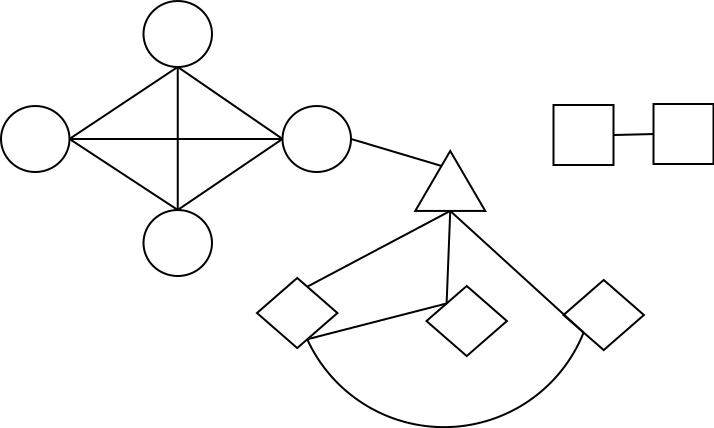
\includegraphics[width=0.7\textwidth]{figures/grafo.png}
\caption{A instância de teste triângulo está ligada ao grafo formado pela classe dos círculos e dos losangos, porém não apresenta ligações com os quadrados.}
\label{fig::grafo}
\end{figure}

Para cada grafo representando uma classe, podemos calcular a credibilidade do exemplo de teste para aquela classe e a incorporar ao classificador Bayesiano. Decidimos modificar a Equação~\ref{eqn::classindependence}, sugerindo seguinte fórmula:

\begin{equation}\label{eqn::nbcredgrafo}
P(X|c_{j}) = \prod^{D}_{i=1}{(P(x_i|c_j)) \cdot (\alpha + Cr_{rel}(X,c_j)) } 
\end{equation}

Como na Equação~\ref{eqn::classindependence}, continuamos calculando o produtório dos atributos que compõem o exemplo $X$, porém calculamos também a credibilidade de $X$ em relação a classe $c_i$. Utilizamos um fator $\alpha$ para evitarmos que a falta de uma aresta entre $X$ e instâncias da classe $i$ possa resultar em uma probabilidade nula de que $X$ seja da classe $i$. Note que poderíamos, sem problema algum, juntar as Equações \ref{eqn::classindependence_conteudo} e \ref{eqn::nbcredgrafo} dando origem a um classificador Bayesiano que leva em conta tanto a credibilidade do conteúdo quanto a dos relacionamentos:

\begin{equation}\label{eqn::nbcredcompleta}
P(X|c_{j}) = \prod^{D}_{i=1}{(P(x_i|c_j) \cdot Cr_{cont}(x_i,c_j)) \cdot (\alpha + Cr_{rel}(X,c_j)) } 
\end{equation}


Pelo fato de modelarmos os relacionamentos existentes entre as entidades por meio de grafos, decidimos por utilizarmos as diversas métricas de redes complexas [cite], a fim de explorarmos as propriedades dos grafos criados. Um exemplo simples de uma dessas métricas é contar o número de vizinhos de um vértice, $viz(v,c_j)$. Essa função retornaria o número de conexões o vértice $v$ tem com seus vizinhos que são da classe $c_j$. Partimos do pressuposto que se um vértice for importante para uma determinada classe $j$, $viz(v,c_j)$, será um valor superior para aquela classe. Na Figura~\ref{fig::grafo}, a classe losango seria a de maior credibilidade para classificarmos o triângulo, baseando nessa métrica. Outras várias métricas importantes podem ser listadas e combinada, sendo assim, atribuímos toda a Seção~\ref{subsec::pg_metricas_grafos} para maiores detalhes.  


%%%%%%%%%%%%%%%%%%%%------------------------------------------------------------------------------------------------------------------------------------%%%%%%%%%%%%%%%%%%%%%%%%%%%%%%%%%
%%%%%%%%%%%%%%%%%%%%------------------------------------------------------------------------------------------------------------------------------------%%%%%%%%%%%%%%%%%%%%%%%%%%%%%%%%%
%%%%%%%%%%%%%%%%%%%%------------------------------------------------------------------------------------------------------------------------------------%%%%%%%%%%%%%%%%%%%%%%%%%%%%%%%%%
%%%%%%%%%%%%%%%%%%%%------------------------------------------------------------------------------------------------------------------------------------%%%%%%%%%%%%%%%%%%%%%%%%%%%%%%%%%

\section{Classificador \textsc{KNN}.}
\label{subsec::cred_knn}

%No decorrer dessa seção, explicaremos o algoritmo dos K vizinhos mais próximos (do inglês, \textit{K-Nearest Neighbor}, KNN). Da mesma forma que fizemos com o \textit{Naïve Bayes}, dedicamos uma seção, Seção~\ref{subsubsec::knn_cred}, exclusivamente para abordarmos o \textsc{KNN} integrado a credibilidade. 

O algoritmo dos $K$ vizinhos mais próximos (\textsc{KNN}) é conhecido por ser um método de aprendizado baseado em analogias, ou seja, comparamos o teste com os exemplos contidos no treinamento a fim de conseguirmos encontrar aqueles com maior semelhança. 
Tipicamente, cada exemplo existente é uma tupla de $D$ dimensões e representa um ponto em um espaço $D$-dimensional. 
Quando um novo exemplo de teste, de classe desconhecida, necessita ser classificado, o algoritmo \textsc{KNN} procura nesse espaço $D$ dimensional pelos $k$ exemplos do treinamento que estão mais perto do teste. 
Por fim, os $k$ vizinhos mais próximos realizam uma votação para escolherem qual será a classe que o teste pertence.
Na Figura~\ref{fig::knn} temos um triângulo que representa nosso exemplo de teste, os quadrados e losangos, representando os exemplos de treinamento pertencentes a classe Quadrado e Losango, respectivamente. As orbitas circulares existentes na figura são epicêntricas e servem apenas para fins didáticos.
Por essa figura, vemos a importância do parâmetro $k$ na decisão da classe que um objeto pertence. Considerando que cada objeto tem o mesmo peso na votação, caso tivéssemos $k=1$, escolheríamos a classe bola para o exemplo de teste, entretanto, se tivéssemos $k=5$, escolheríamos a classe Quadrado. Para valores de $k$ entre 2 e 4, como temos 3 vizinhos a uma mesma distância, temos que considerar algum método de desempate. Em nosso trabalho, ordenamos os vizinhos primeiramente pela distância até o teste e depois por um identificador único. Dessa forma, minimizamos problemas relativos a ordem como os exemplos de treinamento são apresentados.

\begin{figure}[ht!]
\centering
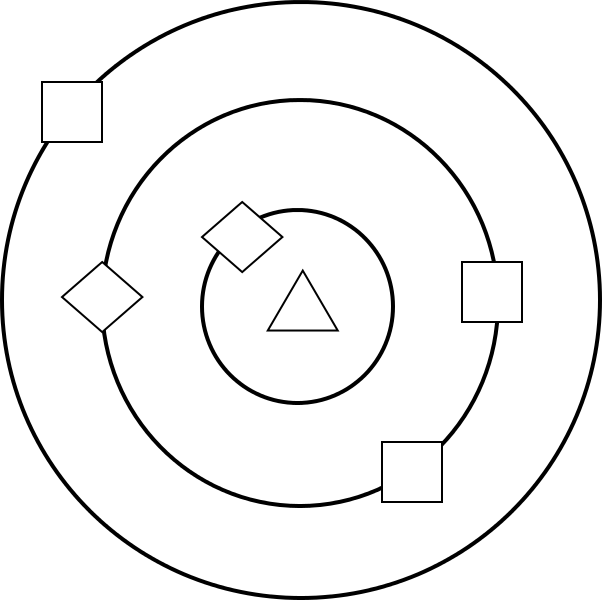
\includegraphics[width=0.5\textwidth]{figures/knn.png}
\caption{O algoritmo dos $k$ vizinhos mais próximos.}
\label{fig::knn}
\end{figure}

Como vimos, uma parte fundamental do \textsc{KNN} é podermos calcular o quão próximo uma instância de teste está das instâncias de treinamento. 
Essa proximidade é tipicamente calculada por uma métrica de distância que pode variar de problema para problema. Neste trabalho, utilizamos 3 métricas diferentes, dependendo se estamos classificando um atributo $A_i$ que seja categórico, numérico ou textual. Para duas instâncias $X_1 =  (x_{11}, x_{21}, x_{31}, ..., x_{D1})$ e $X_2 = (x_{12}, x_{22}, x_{32}, ..., x_{D2})$, nas quais $x_{ij}$ representa o valor do atributo $A_i$ para a instância $j$, temos que, caso $A_i$ seja:

\begin{itemize}

\item numérico, utilizamos a distância Euclidiana:

\begin{equation}\label{eqn::distancia_euclidiana}
    dist(X_1, X_2) =  \sqrt{\sum_{i=1}^D (x_{i1}-x_{i2})^2}
\end{equation}

    Com o intuito de evitar que um atributo com grande escala de valores sobreponha um outro atributo de uma menor escala, empregamos a normalização \textit{min-max} para todos os valores $x_i$ do correspondente atributo $A_i$: 

\begin{equation}\label{eqn::distancia_euclidiana}
    x'_{i} =  \frac{x_{i} - min_{A_i}}{ max_{A_i} - min_{A_i} }
\end{equation}

\item categórico, comparamos $X_1$ e $X_2$ e somamos uma unidade a distância entre as instâncias para cada $x_i$ que tenha valores distintos entre $X_1$ e $X_2$.

\begin{equation}\label{eqn::distancia_cat}
   dist(X_1, X_2) = \sum_{1 < i < D \ \wedge \ x_{i1} \neq x_{i2}} 1.0
\end{equation}

\item textual, tomamos o a distância dos cossenos entre os dois exemplos $X_1$ e $X_2$ e invertemos o seu sinal. Ou seja, sendo $||X_j|| = \sqrt{x_{1j}^2 + x_{2j}^2 + x_{3j}^2 + ... + x_{Dj}^2}$ a norma do vetor representado por um exemplo $X_j$ no espaço e, $x_{ij}$, o peso de um termo $A_i$ no documento $j$, temos que a semelhança entre duas instâncias $X_1$ e $X_2$ pode ser definida como:

\begin{equation}\label{eqn::distancia_texto}
    cosSim(X_1, X_2) = \frac{  x_{i1} \cdot x_{i2} }{ ||X_1|| \cdot ||X_2|| }
\end{equation}

Primeiramente cabe explicar que usamos a métrica \textsc{TFIDF} (\textit{term-frequency - inverse document frequency}), como o peso $x_{ij}$ do termo $A_i$ no documento $j$, mais detalhes sobre a métrica \textsc{TFIDF} na Seção~\ref{subsubsection::tfidf}. Segundo que, como dito, a métrica acima é chamada de semelhança dos cossenos por se basear no ângulo cosseno entre dois vetores no espaço. Como observado, estamos interessados na métrica inversa, logo:
 
 \begin{equation}\label{eqn::distancia_texto}
    dist(X_1, X_2) = - cos_sim(X_1, X_2)
\end{equation}


\end{itemize}

\section{Incorporando a credibilidade no \textsc{KNN}.}
\label{subsubsec::knn_cred}

De forma paralela ao efetuado nas Seções \ref{subsubsec::nbcredconteudo} e \ref{subsubsec::nbcredgrafos}, iremos em um primeiro momento abordar sobre como incorporar ao \textsc{KNN} a credibilidade baseada no conteúdo dos exemplos, Seção \ref{subsubsec::knncredconteudo}. Após isso, na Seção~\ref{subsubsec::knncredgrafos}, analisaremos a credibilidade do ponto de vista das interações entre o exemplo de teste e os exemplos de treinamento, modeladas por meio de grafos.

\subsection{\textsc{KNN} com credibilidade baseada no conteúdo.}
\label{subsubsec::knncredconteudo}


Acoplar a credibilidade no algoritmo \textit{Naïve Bayes} é uma tarefa mais imediata do que incorporá-la ao \textsc{KNN}, isso se deve a maior homogeneidade do algoritmo Bayesiano. Aqui teremos que trabalhar em cada uma das fórmulas separadamente, sendo que, novamente, buscamos uma maneira de quantificar o relacionamento entre um atributo e uma classe. Note que o \textsc{KNN} não realiza essa associação explicitamente, ou seja, como vimos na Seção~\ref{subsec::cred_knn}, somente observamos a classe pertencente a uma instância de treinamento quando já temos os $k$ vizinhos mais próximos definidos e estamos votando para saber qual a classe a ser escolhida.

O \textsc{KNN} é um algoritmo que, de uma maneira geral, compara duas instâncias, uma do conjunto de treinamento e outra do teste, e baseia-se em algum cálculo respectivo a um mesmo atributo $A_i$ de cada uma das instâncias. O que tentamos fazer é utilizar o conhecimento de qual classe a instância de teste pertence e avaliarmos o quanto de credibilidade o valor $x_i$ de um determinado atributo $A_i$ nos provê em relação aquela classe $c_j$ da instância de treino.

Efetivamente, em nossos testes, empregamos a credibilidade para classificação textual e categórica. Embora acreditemos que seja perfeitamente possível utilizarmos o mesmo raciocínio para definirmos a credibilidade em atributos numéricos, deixamos essa tarefa como trabalho futuro. A seguir, nas Seções~\ref{subsubsec::knncat} e~\ref{subsubsec::knntexto}, apresentamos as modificações realizadas no algoritmo dos $k$ vizinhos mais próximos para os atributos categóricos e textuais, respectivamente.

\subsubsection{\textsc{KNN} categórico.}
\label{subsubsec::knncat}

Procuramos, ao desenvolver as modificações seguintes, ter em vista dois fatos importantes:
\begin{enumerate}
\item Se a instância de treinamento e a de teste têm os mesmos valores para todos os seus atributos, então a distância entre as mesmas é zero. 
\item Uma instância de treino que apresenta diferença em $T$ atributos da instância de teste, tende a ter uma distância menor que outra que apresente $T+1$ atributos distintos.
\end{enumerate}

A regra 1 é bastante simples, não criamos uma distância de onde a mesma não existe. A regra 2 diz que ao levar em consideração a classe da instância de treinamento, iremos criar uma pertubação no espaço, porém queremos que essa pertubação seja controlada de forma a continuarmos podendo recorrer à hipótese básica do \textsc{KNN} de que instâncias parecidas, ou seja, com grande número de atributos iguais, estão bem próximas em uma distribuição espacial.

Visualmente, o que queremos com a modificação realizada no algoritmo dos vizinhos mais próximos está expresso na Figura~\ref{fig::KNNantesedepois}. Na Figura~\ref{fig::KNNantesedepois}-(a) temos a situação já discutida anteriormente, composta de um exemplo do treino que difere em uma característica, três que diferem em duas e um outro que difere em três, sendo que esses são os cinco vizinhos mais próximos de nosso exemplo de teste. Por sua vez, na Figura~\ref{fig::KNNantesedepois}-(b) temos os mesmos exemplos mostrados, porém com as distâncias entre o teste e o treino sendo comparadas utilizando o conhecimento sobre a qual classe pertence o exemplo de treino. Pode-se observar que as instâncias da classe Quadrado foram mais afetadas, podendo significar que o exemplo de teste pertença a classe Losango. Dessa vez, ao contrario do que teríamos na situação anterior, para valores de $k$ entre 1 e 3, sabemos definir que o teste pertence a classe dos losangos, sem precisarmos utilizar uma métrica especial de desempate. 

\begin{figure}[ht]
\centering
\subfloat[\textsc{KNN} original]{
    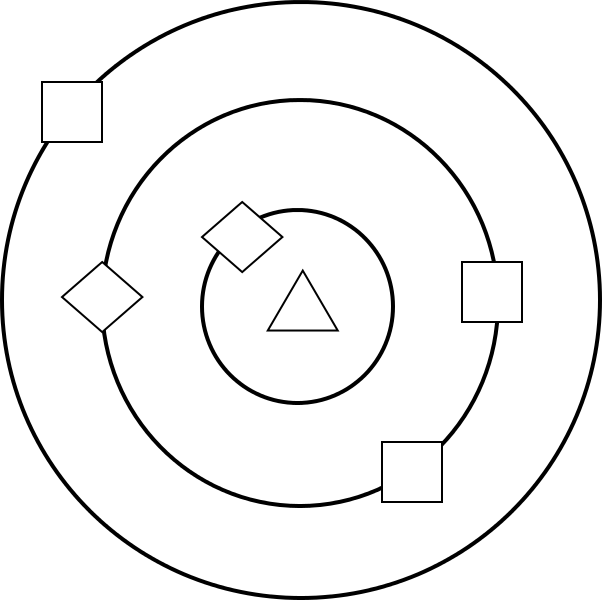
\includegraphics[width=0.5\textwidth]{figures/knn.png}
}
\subfloat[\textsc{KNN} com credibilidade]{
    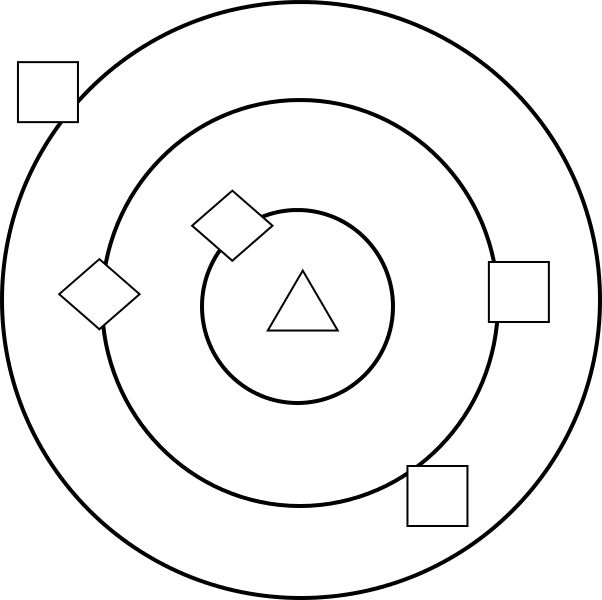
\includegraphics[width=0.5\textwidth]{figures/knncred.png}
}
\caption{Em (a) temos o algoritmo original dos $K$ vizinhos mais próximos e em (b) temos um possível resultado da utilização da credibilidade conjuntamente ao \textsc{KNN}.  
\label{fig::KNNantesedepois}}
\end{figure}

Levando em consideração o que foi mostrado até esse ponto, sendo $X_1$ a instância de teste, $X_2$ a de treino e $c_{X_2}$ a classe a qual nossa instância de treino pertence, modificamos a Equação~\ref{eqn::distancia_cat} para:

\begin{equation} \label{eqn::distancia_cat_cred}
   dist(X_1, X_2) = \sum_{1 < i < D\ \wedge \ x_{i1} \neq x_{i2}} 1.0 + \frac{1.0}{1.0 + Cr_{cont}(x_{i1}, c_{X_2} ))}
\end{equation}

Para estarmos de acordo com o efeito mostrado na Figura \ref{fig::KNNantesedepois}, apenas adicionamos um termo relacionado a credibilidade na Equação~\ref{eqn::distancia_cat}, um fator inversamente proporcional ao valor calculado para a credibilidade. Note que teríamos os mesmos resultados se excluíssemos o primeiro 1.0 existente dentro do somatório da equação acima, porém o que faríamos seria aproximar os exemplos com maior credibilidade ao invés de afastar os com menor.

\subsubsection{\textsc{KNN} textual.}
\label{subsubsec::knntexto}

Decidimos, assim como feito na incorporação da credibilidade nos atributos categóricos, apenas utilizar a credibilidade relacionada ao termo do teste e a classe do exemplo de treinamento. Dessa forma, modificamos a Equação \ref{eqn::distancia_texto}, resultando em:

\begin{equation}\label{eqn::distancia_texto_cat}
    dist(X_1, X_2) = \frac{  Cr_{cont}(x_{i1}, c_{X_2}) \cdot x_{i1} \cdot x_{i2} }{ ||X'_1|| \cdot ||X_2|| }
\end{equation}

Repare que utilizamos $||X'_1||$ como a norma do vetor $X_1$, levando em conta a credibilidade em relação à classe da instância de treino $X_2$, logo teríamos que $||X'_1|| = \sqrt{ ( Cr_{cont}(x_{11}, c_{X_2}) \cdot x_{11} )^2 + ( Cr_{cont}(x_{21}, c_{X_2}) \cdot x_{21} )^2 +  ... +  ( Cr_{cont}(x_{D1}, c_{X_2}) \cdot  x_{D1} )^2}$.
Novamente, assim como discutido na Seção~\ref{subsubsec::nbcredconteudo}, existem diversas métricas que podemos utilizar para inferirmos a credibilidade de um elemento, a fim de melhorarmos a classificação do algoritmo \textsc{KNN}. Algumas dessas métricas já foram previamente discutidas e o serão novamente ao longo desse trabalho. Entretanto, voltamos a frisar que a escolha de uma função de credibilidade é dependente ao contexto que a mesma está inserida e combinar as métricas disponíveis é uma tarefa combinacional cara e, para tanto, estamos usando Programação Genética como será discutido em detalhes no Capítulo~\ref{cap::programacao_genetica}.

\subsection{\textsc{KNN} com credibilidade baseada em relacionamentos.}
\label{subsubsec::knncredgrafos}

Exatamente a mesma situação exposta com detalhes na Seção~\ref{subsubsec::nbcredgrafos} retoma à cena. Ou seja, modelamos a credibilidade atribuída a uma instância de teste em relação a determinada classe utilizando o relacionamento que aquela instância tem com as demais instâncias de treino, levando em consideração a classe que as mesmas pertencem. Diferentemente da modelagem da credibilidade para o conteúdo do algoritmo \textsc{KNN}, dessa vez, podemos criar apenas um modelo que se adapta a qualquer tipo de atributo, numérico, categórico ou textual. Logo, sendo $X_1$ a instância de teste, $X_2$ a instância de treino e $\alpha$ o fator somado a credibilidade de relacionamento para evitarmos valores nulos no denominador, temos:

\begin{equation}\label{eqn::distancia_grafos}
%    dist(X_1, X_2) = dist(X_1, X_2) \cdot (\alpha + Cr_{rel}(X_1, class_{X_2})) 
    dist(X_1, X_2) = \frac{ dist(X_1, X_2) } { \alpha + Cr_{rel}(X_1, class_{X_2}) }
\end{equation}

Note que estamos modificando o valor da distância calculado entre a instância de teste e a de treino, baseando no fato que quanto maior a credibilidade do relacionamento do teste $X_1$ a uma classe $c_i$, menor será a distância entre o exemplo $X_1$ e os outros exemplos do treinamento que pertencem a classe $c_i$.

Mais uma vez, podemos utilizar as várias propriedades dos grafos para calcularmos a credibilidade dos relacionamentos. Na Seção~\ref{subsec::pg_metricas_grafos} definimos várias métricas que calculam essas propriedades. Por fim, usamos a Programação Genética para combinarmos essas métricas a fim de obtermos uma melhor função de credibilidade que explore o melhor possível o relacionamento exemplo-classe.



%-------------------------------------------------------------

\chapter{Modelando a Credibilidade com Programação Genética}
\label{cap::programacao_genetica}

\section{Programação Genética}

\subsection{Operadores}

\subsection{Fitness}


\section{Credibilidade baseada no Conteúdo}
\label{sec::pg_cred_baseada_conteudo}

Nessa seção apresentamos várias métricas utilizadas na construção dos indivíduos usados pelo Programa Genético. Elas foram modeladas diferentemente para os casos nos quais os atributos são textuais ou categóricos, sendo que a modelagem para atributos numéricos foi deixada como trabalho futuro. Em suma, métricas que realizam cálculos baseados em frequência de termos e documentos não puderam ser usadas para atributos categóricos, porém todas as demais foram. Dessa forma, na Seção~\ref{subsec::pg_metricas_conteudo_textual} temos as métricas que foram modeladas única e exclusivamente para serem utilizadas na tarefa de classificação de textos e na Seção~\ref{subsec::pg_metricas_conteudo} temos as métricas que foram estendidas e estão sendo usadas para classificação categórica, além da textual.

\subsection{Métricas Modeladas Para Atributos Textuais Exclusivamente.}
\label{subsec::pg_metricas_conteudo_textual}

As métricas usadas para atributos textuais consistem em algumas variantes do \textit{TFIDF}, métrica mais difundida entre as apresentadas. Na tabela~\ref{table::metricas_textuais}, temos apresentados algumas expressões amplamente utilizadas nas métricas aqui listadas.

\begin{table}[ht*]
\centering
\begin{tabular}{|c|c|}
\toprule
    \textbf{Expressão} & \textbf{Explicação} \\
\midrule
    $N$           & Número de documentos na base de treinamento. \tabularnewline \hline
    $M$           & Número de classes da coleção. \tabularnewline \hline
    $DF_{x_i} $   & Número de documentos do conjunto do treino que contém o termo $x_i$. \tabularnewline \hline
    $DF_{x_ic_j}$ & Número de documentos do treino com o termo $x_i$ e pertencentes a classe $c_j$. \tabularnewline \hline
    $CF_{x_i}$    & Número de classes em que o termo $x_i$ ocorre. \tabularnewline \hline 
    $F_{x_i}$     & Número de vezes que o termo $x_i$ aparece nos documentos de treinamento. \tabularnewline \hline
    $F_{x_ic_j}$  & Número de vezes que o termo $x_i$ aparece em documentos da classe $c_j$ no treino. \tabularnewline 
\bottomrule
\end{tabular}
\caption{Explicação das principais expressões utilizadas para definição das métricas para atributos textuais.}
\label{table::metricas_textuais}
\end{table}


%%%%%%%%%%%%%%%%%%%-------------------------------------------------------%%%%%%%%%%%%%%%%%%%%%%%%%%%%%%%%%%%%%%%%
\subsubsection{Frequência do Termo (TF)}
\label{subsubsection::sumtf}

A frequência de um termo, \textit{TF} da expressão em inglês, \textit{Term Frequency}, é simplesmente o número de vezes que um termo aparece na coleção de treinamento. Utilizamos o logaritmo desse valor como um fator normalizador, para evitar que termos muito frequentes dominem a função de credibilidade:
\begin{equation}\label{eqn::sumtf}
   TF(x_i) = 1.0 + \log{ ( F_{x_i} ) }
\end{equation}


%%%%%%%%%%%%%%%%%%%-------------------------------------------------------%%%%%%%%%%%%%%%%%%%%%%%%%%%%%%%%%%%%%%%%
\subsubsection{Frequência do Termo por Classe (TFClasse)}
\label{subsubsection::tf}

A frequência de um termo em uma classe, \textit{TFClasse}, segue o mesmo padrão utilizado pela métrica \textit{TF}, porém dessa vez contamos apenas os termos que aparecem em uma dada classse $c_j$:
\begin{equation}\label{eqn::tf}
   TFClasse(x_i, c_j) = 1.0 + \log{ ( F_{x_ic_j} ) }
\end{equation}


%%%%%%%%%%%%%%%%%%%-------------------------------------------------------%%%%%%%%%%%%%%%%%%%%%%%%%%%%%%%%%%%%%%%%
\subsubsection{Frequência dos Documentos por Termo (DF)}
\label{subsubsection::df}

A métrica \textit{DF}, do inglês, \textit{Document Frequency}, procura analisar a importância de um termo em relação ao número de documentos que o mesmo aparece:
\begin{equation}\label{eqn::df}
   DF(x_i) = 1.0 + \log{ ( DF_{x_i} ) }
\end{equation}


%%%%%%%%%%%%%%%%%%%-------------------------------------------------------%%%%%%%%%%%%%%%%%%%%%%%%%%%%%%%%%%%%%%%%

\subsubsection{Frequência de Documentos por Termo-Classe (DFClasse)}
\label{subsubsection::sumdf}

A métrica \textit{DFClasse} apenas avalia o número de documentos que um termo aparece em relação a uma classe específica, tentando capturar a importância de um termo para uma classe em relação ao número de documentos onde aquele termo está presente:
\begin{equation}\label{eqn::sumtf}
   DFClasse(x_i,c_j) = 1.0 + \log{ ( DF_{x_ic_j} ) }
\end{equation}


%%%%%%%%%%%%%%%%%%%-------------------------------------------------------%%%%%%%%%%%%%%%%%%%%%%%%%%%%%%%%%%%%%%%%
\subsubsection{Inverso da Frequência de Documentos (IDF)}
\label{subsubsection::idf}

O Inverso da Frequência de Documentos, \textit{IDF} do inglês \textit{Inverse Document Frequency}, é uma conhecida métrica que avalia a popularidade de um determinado termo em um conjunto de documentos. Temos que quanto mais popular é um termo ao longo dos documentos de uma coleção, pior é sua capacidade de discriminação, logo:
\begin{equation}\label{eqn::tficf}
   IDF(x_i) = \log( \frac{|N|} {DF(x_i)} )
\end{equation}

%%%%%%%%%%%%%%%%%%%-------------------------------------------------------%%%%%%%%%%%%%%%%%%%%%%%%%%%%%%%%%%%%%%%%

\subsubsection{Inverso da Frequência de Documentos por Classe (IDFClasse)}
\label{subsubsection::idf}

O Inverso da Frequência de Documentos por classe, \textit{IDFClasse} é uma versão do \textit{IDF} em selecionamos somente documentos de uma dada classe:
\begin{equation}\label{eqn::tficf}
   IDFClasse(x_i,c_j) = \log( \frac{DF_{c_j}} {DF(x_ic_j)} )
\end{equation}


%%%%%%%%%%%%%%%%%%%-------------------------------------------------------%%%%%%%%%%%%%%%%%%%%%%%%%%%%%%%%%%%%%%%%

\subsubsection{Frequência do Termo Inverso da Frequência de Documentos (TFIDF)}
\label{subsubsection::tfidf}

Uma das métricas de pesos para atributos em classificação de textos mais populares na literatura é o \textit{TFIDF} (do inglês, \textit{Term Frequency Inversed Document Frequency}), ver \cite{Salton88}. O \textit{TFIDF} combina a frequência de um termo (\textit{Term Frequency}) que assume que múltiplas aparições de um termo em um documento é mais importante que aparições únicas com o inverso da frequência de um documento (\textit{Inverded Document Frequency}) que diz que termos raros são de maior poder discriminativo que termos muito frequentes. Em síntese, a fórmula de TFIDF é nada mais que a multiplicação das métricas TF e IDF, como já esperávamos:
\begin{equation}\label{eqn::tficf}
   TFIDF(x_i, c_j) =  F_{x_ic_j} \cdot \log( \frac{DF_{c_j}}{ DF_{x_ic_j} } )
\end{equation}

%%%%%%%%%%%%%%%%%%%-------------------------------------------------------%%%%%%%%%%%%%%%%%%%%%%%%%%%%%%%%%%%%%%%%
\subsubsection{Frequência do Termo Inverso da Frequência da Classe (TFICF)}
\label{subsubsection::tficf}

O TFICF (do inglês, \textit{Term Frequency Inversed Class Frequency}) é uma variação do esquema TFIDF (ver Seção~\ref{subsubsection::tfidf}). Novamente, TF se refere a quanto importante é um termo em uma classe, pois trata-se de sua frequência; por sua vez, ICF é interpretado como a frequência relativa de um termo em uma classe. Como é possível observar, não existe uma forma de diferenciarmos entre um termo que aparece frequentemente em um pequeno subconjunto de documentos e um termo que está presente em um grande número de documentos entre as classes. Como mostrado por~\cite{ChihHow04}, a fórmula para TFICF é:
\begin{equation}\label{eqn::tficf}
   TFICF(x_i, c_j) = N_{x_ic_j} \cdot \log( \frac{M}{CF_{x_i}} )
\end{equation}

%%%%%%%%%%%%%%%%%%%-------------------------------------------------------%%%%%%%%%%%%%%%%%%%%%%%%%%%%%%%%%%%%%%%%
\subsubsection{Category Term Description}
\label{subsubsection::ctd}

Definido por~\cite{ChihHow04}, \textit{Category Term Description} é uma métrica de seleção de atributos para classificação textual baseada em TFIDF (Seção~\ref{subsubsection::tfidf}) e TFICF (Seção~\ref{subsubsection::tficf}). How et al. propõe uma melhoria ao TDICF acreditando que quanto menos um termo ocorre entre os documentos, maior o poder discriminativo daquele termo, logo:
\begin{equation}\label{eqn::cdt}
   CDT(x_i, c_j) = TFClass(x_i, c_j) \cdot ICF(x_i, c_j) \cdot IDFClass(x_i,c_j)
\end{equation}

%%%%%%%%%%%%%%%%%%%-------------------------------------------------------%%%%%%%%%%%%%%%%%%%%%%%%%%%%%%%%%%%%%%%%
\subsubsection{Dominância}
\label{subsubsection::dom}

Dominância é uma métrica originalmente proposta em~\cite{Zaiane02} e utilizada mais recentemente no trabalho de~\cite{Rocha08} para criação do que foi chamado de janela temporal de um documento. Em suma, utilizado exclusivamente em classificação textual, o método normaliza a frequência de um documento em um classe por todas as classes existentes, logo:

\begin{equation}\label{eqn::dom}
   Dominancia(x_i, c_j) = \frac{ DF_{x_ic_j} } { \sum\limits_{c_k \in \mathbb{C}} DF_{ x_ic_k } } 
\end{equation}

\subsubsection{MaxTFIDF}
\label{subsubsection::maxtfidf}

\subsubsection{MaxTFICF} 
\label{subsubsection::maxtficf}

\subsubsection{MaxCTD}
\label{subsubsection::maxctd}

\subsubsection{MaxDom}
\label{subsubsection::maxdom}



\subsection{Métricas Modeladas Para Atributos Textuais e Categóricos.}
\label{subsec::pg_metricas_conteudo}


Todas as métricas apresentadas nessa seção foram utilizadas para geração de uma função de credibilidade tanto para atributos textuais quanto para os categóricos. Elas são inspiradas em probabilidades que podem ser facilmente calculadas dos exemplos contidos no conjunto de treinamento. Destacamos que a probabilidade condicional $P(x_i|c_j)$ é a principal métrica, pois as demais, complexas ou não, são derivações dessa. Pretendemos através da Tabela~\ref{table::metricas_textuais_categoricos} mostrar as definições utilizadas para definição dos atributos categórico, lembrando que quando se trata de um problema de classificação de texto deve-se recorrer a Tabela~\ref{table::metricas_textuais}.


\begin{table}[ht*]
\centering
\begin{tabular}{|c|c|}
\toprule
    \textbf{Métrica} & \textbf{Explicação} \\
\midrule
    $N$           & Número de exemplos na base de treinamento. \tabularnewline \hline
    $M$           & Número de classes da coleção. \tabularnewline \hline
    $F_{x_ic_j}$  & Número de vezes que temos o atributo $A_i$ com o valor $x_i$ em exemplos da classe $c_j$. \tabularnewline \hline
    $F_{c_j}$     & Número de vezes que o atributo $A_j$ assume o valor $x_i$ em exemplos da classe $c_j$. \tabularnewline 
\bottomrule
\end{tabular}
\caption{Explicação das principais expressões utilizadas para definição das métricas para atributos categóricos.}
\label{table::metricas_textuais_categoricos}
\end{table}

%%%%%%%%%%%%%%%%%%%-------------------------------------------------------%%%%%%%%%%%%%%%%%%%%%%%%%%%%%%%%%%%%%%%%
\subsubsection{Medida de Ambiguidade (AM)}
\label{subsubsection::am}

A medida de ambiguidade (AM de \textit{Ambiguity Measure}) foi definida por~\cite{Mengle08} e utilizada como um método de seleção de atributos. Ela atribui valores maiores para os atributos considerados menos ambíguos, onde um atributo é não ambíguo quando sua presença indica com um alto grau de confiança que o exemplo pertence a uma classe específica. Podemos calcular $AM(x_i, c_j)$ como:
\begin{equation}\label{eqn::am}
   AM(x_i, c_j) = \frac{ N_{x_{i}c_{j}}}{\sum\limits_{c_k \in \mathbb{C}} N_{x_{i}c_{k}}}.
\end{equation}

%%%%%%%%%%%%%%%%%%%-------------------------------------------------------%%%%%%%%%%%%%%%%%%%%%%%%%%%%%%%%%%%%%%%%
\subsubsection{Probabilidade Condicional ($P(x_i|c_j)$)}
\label{subsubsection::pc}

A probabilidade condicional $P(x_i|c_j)$ provém do algoritmo \textit{Naïve Bayes} como foi discutido na Seção~\ref{subsec::cred_nb}.
Temos dois modos de calcular $P(x_i|c_j)$, um para quando temos $A_i$ categórico e outro para quando estamos realizando classificação textual.
A ideia principal de ambos é a mesma, para uma dada classe $c_j$, calculamos a probabilidade do atributo $A_i$ ter o valor $x_i$ entre todos possíveis. 
Para classificação categórica, basta apenas contar quantas vezes $A_i$ vale $x_i$ para uma dada classe $c_j$:
    \begin{equation}\label{eqn::nbcattexto}
        P(x_i|c_j) = \frac{ N_{x_{i}c_{j}} }{ N_{c_{j}} } 
    \end{equation}
%Onde $N_{x_{i}c_{j}}$ é o número de vezes que temos o termo $x_i$ nos exemplos de treino da classe $c_j$ e $N_{c_{j}}$ é o número de exemplos de treino da classe $c_j$.
        
Para classificação textual, contamos quantas vezes um termo aparece em uma classe em comparação a todos os termos possíveis:
    \begin{equation}\label{eqn::nbcattexto}
        P(x_i|c_j) = \frac{ N_{x_{i}c_{j}} }{ \sum\limits^{D}_{k = 1} {  N_{x_{k}c_{j}}} } 
    \end{equation}
%Onde $N_{x_{i}c_{j}}$ é o número de vezes que temos o termo $x_i$ nos documentos de treino da classe $c_j$ e $D$ é o número o vocabulário conhecido no treino.

%%%%%%%%%%%%%%%%%%%-------------------------------------------------------%%%%%%%%%%%%%%%%%%%%%%%%%%%%%%%%%%%%%%%%
\subsubsection{Inverso da Probabilidade Condicional ($P(x_i|c_j)$)}
\label{subsubsection::pc'}
Com o inverso da probabilidade condicional, calculamos a probabilidade de um atributo $A_i$ não valer $x_i$ para uma classe $c_j$. Podemos realizar esse calculo apenas com a seguinte fórmula:
\begin{equation}\label{eqn::plinhattalquec}
   P(\overline{x_i}|c_j) = 1.0 - P(x_i|c_j)
\end{equation}

%%%%%%%%%%%%%%%%%%%-------------------------------------------------------%%%%%%%%%%%%%%%%%%%%%%%%%%%%%%%%%%%%%%%%
\subsubsection{Índice de Gini melhorado (GINI)}
\label{subsubsection::gini}

O índice de Gini é uma métrica baseada na curva de Lorenz que mostra a função de distribuição acumulada de uma variável. Esse índice é amplamente utilizado nas Ciências Econômicas como uma métrica para avaliação da distribuição de renda pela população de um certo país ou região. Infelizmente por essa métrica, o Brasil é um dos países mais desiguais do mundo (ver \cite{cia-gini}). 
Baseado na ideia de desigualdade, podemos pensar na distribuição de um atributo nas M classes possíveis. Um atributo que seja desigualmente distribuído é certamente um atributo com um maior poder de discriminação, e portanto, um atributo mais importante. O trabalho de~\cite{Shang07} consistiu na criação de um selecionador de atributos para classificadores textuais baseando-se no Índice de Gini, chamado Índice de Gini melhorado. Ao contrario da maioria das métricas expostas nessa seção, o Índice de Gini melhorado tem apenas um parâmetro, o valor do $i$-ésimo atributo, não levando em consideração nenhuma classe específica. Ele é considerado melhorado por algumas pequenas diferenças com o método tradicional de Gini, entre elas o fato de um maior valor se referir a um melhor atributo e não ao contrário como é feito no método original. A fórmula sugerida por \cite{Shang07} para ser utilizada em classificação de atributos textuais é dada por:
\begin{equation}\label{eqn::gini}
   GINI(x_i) = \sum\limits_{c_k \in \mathbb{C}} P(x_i|c_k)^2 \cdot P(c_k|x_i)^2
\end{equation}
Shang et al. destaca o fato da não utilização do fator $P(x_i)$, fazendo com que o Índice de GINI melhorado sofra menos a influência de atributos frequentes conseguindo capturar a capacidade de um atributo ser importante para distinguir uma classe, independente de qual classe é. Destacamos que $P(c|x_i)$ é justamente a probabilidade que o algoritmo Bayesiano pretende calcular, logo aproximamos esse fator como:
\begin{equation}\label{eqn::gini}
   P(c_j|x_i) = \frac{  P(c_j \wedge x_i) } { P(x_i) } = \frac{ \frac{ N_{x_ic_j}}{  \sum\limits_{c \in \mathbb{C}} \sum\limits_{k=1}^{D} {Nx_kc}  } } { \frac{\sum\limits_{c \in \mathbb{C}} N_{x_ic}}{ \sum\limits_{c \in \mathbb{C}} \sum\limits_{k=1}^{D} {Nx_kc}}} = \frac{ N_{x_{i}c_{j}}}{\sum\limits{c_k \in \mathbb{C}} N_{x_{i}c_{k}}}.
\end{equation}
Que é o mesmo valor definido por~\cite{Mengle08} para a métrica Medida da Ambiguidade mostrada na Seção~\ref{subsubsection::am}.

%%%%%%%%%%%%%%%%%%%-------------------------------------------------------%%%%%%%%%%%%%%%%%%%%%%%%%%%%%%%%%%%%%%%%
\subsubsection{Ganho de Informação}
\label{subsubsection::ig}

O Ganho de Informação (\textit{Information Gain}, IG), \cite{Yang97}, mede a diminuição da entropia quando um atributo é usado ou não. A entropia é uma medida utilizada no campo da Ciência da Informação que tenta quantificar a desordem, a imprevisibilidade. Quanto maior a entropia maior a entropia, mais difícil é prever um resultado, portanto a métrica IG seleciona os atributos que diminuam o valor da entropia, facilitando descobrir a qual classe um exemplo pertence. O Ganho da Informação pode ser calculado da seguinte forma:
\begin{equation}\label{eqn::ig}
   IG(x_i, c_j) = \sum_{c \in \{c_j, \overline{c_j}\}}\sum_{x \in \{x_i, \overline{x_i}\}}P(x|c)\log_2\frac{P(x|c)}{P(x)P(c)}.
\end{equation}

%%%%%%%%%%%%%%%%%%%-------------------------------------------------------%%%%%%%%%%%%%%%%%%%%%%%%%%%%%%%%%%%%%%%%
\subsubsection{Cross Entropy}
\label{subsubsection::}

\textit{Cross Entropy} (CE), assim como o Índice de Gini Melhorado, Seção~\cite{subsubsection::gini}, apresenta apenas um parâmetro, um atributo. Novamente aproximamos o calculamos $P(c|x_i)$, pois esse já é o resultado do algoritmo \textit{Naïve Bayes} e, portanto, não o teríamos enquanto estamos calculando a credibilidade de um atributo em relação a uma classe. Assim como enunciado por~\cite{Koller97} e adaptado para seleção de atributos em~\cite{Mladenic98}, essa métrica assume a seguinte fórmula:
\begin{equation}\label{eqn::ce}
   CE(x_i) =  P(x_i) \cdot \sum_{c \in \mathbb{C}} P(c|x_i) \cdot \log_2 \frac{ P(c|x_i) } { P(c) }
\end{equation}

%%%%%%%%%%%%%%%%%%%-------------------------------------------------------%%%%%%%%%%%%%%%%%%%%%%%%%%%%%%%%%%%%%%%%
\subsubsection{CHI-Quadrado}
\label{subsubsection::chi}

O teste \textit{CHI-quadrado - $\chi^2$} é utilizado no campo da Estatística para testar a independência entre dois eventos. Quando usado para seleção de atributos, tipicamente temos que os dois eventos são a ocorrência de uma classe e a ocorrência de um atributo $A_i$ com valor $x_i$, ver~\cite{Zheng03}. Logo,
\begin{equation}\label{eqn::chi}
   CHI(x_i, c_j) = N \cdot \frac{ [ P(x_i|c_j) \cdot P(\overline{x_i}|\overline{c_j}) - P(x_i|\overline{c_j}) \cdot P(\overline{x_i}|c_j) ]^2 } {P(x_i) \cdot P(\overline{x_i}) \cdot P(c_j) \ \cdot P(\overline{c_j}) }
\end{equation}
%como $P(x_i|c_j)$ a probabilidade de termos o atributo $A_i$ com valor $x_i$ dada a classe $c_j$ para classificação categórica e a probabilidade de um documento ter o termos $x_i$ dado que ele pertence a classe $c_j$. Valores próximos de zero indicam a falta de relação entre $x_i$ e $c_j$.

%%%%%%%%%%%%%%%%%%%-------------------------------------------------------%%%%%%%%%%%%%%%%%%%%%%%%%%%%%%%%%%%%%%%%
\subsubsection{Coeficiente de Correlação}
\label{subsubsection::cc}

O Coeficiente de Correlação (CC) é uma métrica de seleção de atributos, variante da métrica \textit{CHI-Quadrada - $\chi^2$}, ver Seção~\ref{subsubsection::chi}. Definida por~\cite{Ng97}, temos que $(CC)^2 = \chi^2$, logo:
\begin{equation}\label{eqn::ce}
   CC(x_i, c_j) = \sqrt{N} \cdot \frac{ P(x_i|c_j) \cdot P(\overline{x_i}|\overline{c_j}) - P(x_i|\overline{c_j}) \cdot P(\overline{x_i}|c_j) } {\sqrt{ P(x_i) \cdot P(\overline{x_i}) \cdot P(c_j) \ \cdot P(\overline{c_j}) } }.
\end{equation}
como a mesma definição de $P(x_i|c_j)$ usada para a métrica $\chi^2$. Os valores positivos para CC correspondem a pertinência do valor de um atributo a uma classe, enquanto valores negativos indicam a não pertinência. Quanto mais positivo (negativo) são os valores de CC, mais fortemente o atributo é relacionado (não relacionado) a uma classe. Para fins de seleção de atributo, valores mais elevados de CC são os mais interessantes, pois mostram uma correlação positiva entre um atributo e uma classe. Em contraste com CC, $\chi^2$ também considera importantes correlações negativas entre atributos e classes, o que acaba resultando que atributos que fortemente indicam a falta de pertinência a uma classe são tão importantes quanto os que indicam.

%%%%%%%%%%%%%%%%%%%-------------------------------------------------------%%%%%%%%%%%%%%%%%%%%%%%%%%%%%%%%%%%%%%%%
\subsubsection{Coeficiente GSS}
\label{subsubsection::gss}
O coeficiente Galavotti–Sebastiani–Simi (GSS) introduzido por~\cite{Galavotti00} é bastante similar a $\chi^2$, Seção~\ref{subsubsection::chi}, e pode ser definido como:
\begin{equation}\label{eqn::gss}
   GSS(x_i, c_j) = P(x_i|c_j) \cdot P(\overline{x_i}|\overline{c_j}) - P(x_i|\overline{c_j}) \cdot P(\overline{x_i}|c_j).
\end{equation}
%sendo $P(x_i|c_j)$ definido na Seção~\ref{subsubsection::pc}. Da mesma forma como o Coeficiente de Correlação, Seção~\ref{subsubsection::cc}, valores positivos correspondem à pertinência de um atributo a uma categoria e, negativos, à não pertinência. 


%%%%%%%%%%%%%%%%%%%-------------------------------------------------------%%%%%%%%%%%%%%%%%%%%%%%%%%%%%%%%%%%%%%%%
\subsubsection{Razão de Chances - \textit{Odds Ratio} (OR)}
\label{subsubsection::or}

Proposta originalmente por~\cite{Rijsbergen79}, a métrica Razão de Chances, do inglês \textit{Odds Ration} (OR), também é uma métrica de seleção de atributos. A ideia básica é que a distribuição de atributos em exemplos relevantes é diferente da distribuição de atributos em exemplos não relevantes. Isso quer dizer que poderíamos definir dois eventos A e B e calculamos a probabilidade de ocorrência de A dividida pela probabilidade de não ocorrência de A e a comparamos com a probabilidade ocorrência de B dividida pela probabilidade de não ocorrência de B:
\begin{equation}\label{eqn::or}
   OR(A, B) = \frac{\frac{A}{1-A}} {\frac{B}{1-B}} = \frac{ A \cdot ( 1 - B )} { B \cdot ( 1 - A ) } .
\end{equation}
Uma razão de chances de 1.0 indica que ocorrer A ou B é igualmente provável, uma razão maior do que 1.0 indica que ocorrer A é mais provável, enquanto que uma razão de chances menor do que 1 indica que o evento B é tem uma probabilidade maior de ocorrer.

A razão de chances tem sido utilizada para selecionamento de atributos por \cite{Mladenic98} fazendo com que A seja $P(x_i|c_j)$ e B seja $P(x_i,\overline{c_j})$. Logo,
\begin{equation}\label{eqn::or}
   OR(x_i, c_j) = \frac{ P(x_i|c_j) \cdot [ 1.0 - P(x_i|\overline{c_j}) ] }{ [ 1.0 - P(x_i|c_j) ] \cdot P(x_i|\overline{c_j})}.
\end{equation}
%em que $P(x_i, c_j)$ é a probabilidade de termos o atributo $A_i$ com valor $x_i$ em exemplos que pertencem a classe $c_j$ e $P(x_i|\overline{c_j})$ é a probabilidade de termos $x_i$ em outras classes que não sejam $c_j$.

\subsubsection{MaxAM}
\label{subsubsection::maxam}

\subsubsection{MaxIG}
\label{subsubsection::maxig}

\subsubsection{MaxCHI}
\label{subsubsection::maxchi}

\subsubsection{MaxCC}
\label{subsubsection::maxcc}

\subsubsection{MaxOR}
\label{subsubsection::maxor}

\subsubsection{MaxGSS}
\label{subsubsection::maxgss}


\section{Credibilidade baseada em Grafos}
\label{sec::pg_cred_baseada_grafos}

\subsection{Métricas modeladas.}
\label{subsec::pg_metricas_grafos}

asdfsad


\subsubsection{NeighborhoodSize3(id,className,graphId)}
\label{subsubsection::neighborhoodsize}

break;
%\subsubsection{getHubScore(id, className, graphId)}
%break;
%QUAL A TRADUCAO DE HUB?


\subsubsection{Closeness}
\label{subsubsection::closeness}

De maneira intuitiva, dizemos que dois objetos estão próximos se eles estão a uma distância arbitrariamente pequena um do outro. Muitas vezes, entretanto, não é fácil estipular o que vem a ser uma distância pequena. Em teoria dos grafos, medimos a distância entre os vértices utilizando o calculo conhecido como caminho mínimo que conta o número mínimo de vértices que necessitamos atravessar para ligar dois vértices escolhidos em um grafo. \textit{Closeness} é uma métrica que calcula a proximidade de um vértice $v$ em relação a todo o grafo usando a média dos caminhos mínimos de $v$ para todos os outros vértices alcançáveis a partir de $v$, ver~\cite{Beauchamp65}. Dessa forma, podemos medir a importância de um vértice calculando quanto tempo em média é gasto para uma informação se espalhar a partir de um vértice $v$ para todo o resto do grafo. Por fim, são considerados vértices mais ``próximos'' aqueles que minimizam esse tempo.

\subsubsection{Betweenness}
\label{subsubsection::constraint}
A métrica de centralidade denominada \textit{Betweenness} se baseia no fato que um vértice é importante em um grafo se ele está entre o caminho de outros vértice, ou seja, um vértice é importante por estar sempre conectando outros vértices em um grafo. O algoritmo do caminho mínimo é o que se utiliza para percorrer da melhor maneira possível uma dada distância em um grafo e portanto, \textit{betweenness} calcula a importância de um vértice contando quantas vezes aquele vértice participa do caminho mínimo entre quaisquer dois outros vértices do grafo em questão, ver~\cite{Sabidussi66}. Obviamente, um vértice central que está no caminho mínimo de vários outros tem mais acesso a informação que circula pelo grafo que um vértice periférico com poucas ligações.

\subsubsection{Eigenvector Centrality}
\label{subsubsection::eigenvector}
A centralidade do Autovetor, em inglês \textit{Eigenvector Centrality}, também é uma medida de centralidade que avalia a importância de um vértice em todo o grafo. Ela atribui valores aos vértices baseados nas conexões que os mesmos têm, sendo que um vértice ganhará uma importância maior se estiver conectado a vértices de maior importância. De maneira matemática, dado que $x_i$ é o valor atribuído ao vértice $i$ e que podemos montar a matriz de adjacência $A$ com os $N$ vértices do grafo, na qual $A_{ij} = 1$ se existe uma aresta entre $i$ e $j$ e $A_{ij}=0$, caso contrário, temos:
\begin{equation}\label{eqn::eigenvector1}
   x_i = \frac{1}{\lambda} \cdot \sum\limits_{j=1}^{N} A_{ij} \cdot x_j
\end{equation}
Que pode ser rescrita utilizando vetores como:
\begin{equation}\label{eqn::eigenvector2}
   X = \frac{1}{\lambda} AX  \;\; \Longleftrightarrow\;\;  AX = \lambda X
\end{equation}
Onde $X$ é dito ser o \textit{autovetor} formado pelos valores de $x_i$ com $0 \leq i \leq N$ e associado ao \textit{autovalor} $\lambda$.  Podem existir muitos valores para $\lambda$ para os quais a Equação~\ref{eqn::eigenvector2} possui solução. Entretanto se utilizarmos todos os valores do \textit{autovetor} como positivos, teremos um único e maior possivel valor para o \textit{autovetor}, ver~\cite{Newman10}. Vale resaltar que o algoritmo \textit{PageRank}, Seção~\ref{subsubsection::pagerank}, é uma variação desse.


\subsubsection{Hub e Autoridade de Kleinberg (Hub e Auth)}
\label{subsubsection::hub}
As métricas conhecidas como Hub e Autoridade de Kleinberg são provenientes do trabalho de~\cite{Kleinberg99}. Elas também são conhecidas pelo nome de algoritmo \textit{Hyperlink-Induced Topic Search} (HITS) e por serem predecessoras do algoritmo \textit{PageRank}, Seção~\ref{subsubsection::pagerank}. Em suma, na \textit{Web}, algumas páginas são conhecidas como \textit{hubs} por não serem especialistas em nenhum assunto específico, mas possuírem ligações para vários outras páginas que são especialistas em seus respectivos assuntos, sendo, portanto, \textit{autoridades} no assunto tratado. Logo, o que temos é que um bom \textit{hub} é representado por uma página (vértice, no grafo que a \textit{Web} representa) que aponta para várias autoridades e uma boa autoridade é aquela apontada por vários \textit{hubs}. Uma página com poucas ligações e com poucas referências não é nem um bom \textit{hub} e nem uma boa autoridade.

\subsubsection{getPageRank(id, className, graphId)}
\label{subsubsection::pagerank}
break;



\subsubsection{getStrength(id, className, graphId)}
\label{subsubsection::strength}
break;

\subsubsection{Burt's Constraint}
\label{subsubsection::constraint}
\cite{Burt04}
break;

\subsubsection{getBibCoupling(id, className, graphId)}
break;
\subsubsection{getCoCitation(id, className, graphId)}
break;
\subsubsection{getJaccardSimilarity(id, className, graphId)}
break;
\subsubsection{getDiceSimilarity(id, className, graphId)}
break;
\subsubsection{getInverseLogSimilarity(id, className, graphId)}
break;
\subsubsection{getAvgNearstNeighborDegree(id, className, graphId)}
acho que nao to uando



%-------------------------------------------------------------
\chapter{Experimentos}
\label{cap::experimentos}
%
\chapter{Experimentos}
\label{cap::experimentos}

\newcommand{\triangOK}{\textcolor[rgb]{00,0.45,0.10}{$\blacktriangle$}}
\newcommand{\triangBAD}{\textcolor[rgb]{0.7,00,00}{$\blacktriangledown$}}
\newcommand{\ball}{\textcolor[rgb]{0.7,0.70,0.0}{$\bullet$}}
 	
%\begin{table}
%\centering
%\begin{footnotesize}
%\toprule
%Tabela
%\midrule
%\bottomrule

%\caption{}
%\label{tab::}
%\end{footnotesize}
%\end{table}


\begin{table}
\centering
\begin{footnotesize}
\begin{tabular}{|c||c|c|}
\toprule
\textbf{Bases} & \textbf{Micro$F_1$} & \textbf{Macro$F_1$}\tabularnewline
\midrule
ACM & 73.62 \textpm{} 0.91 & 57.26 \textpm{} 0.93\tabularnewline
\hline 
20NG & 84.94 \textpm{} 0.58 & 83.68 \textpm{} 0.82\tabularnewline
\hline 
Ohsumed & 66.56 \textpm{} 0.66 & 54.76 \textpm{} 1.27\tabularnewline
\hline 
Reuters & 93.13 \textpm{} 0.29 & 81.96 \textpm{} 1.44\tabularnewline
\bottomrule
\end{tabular}
\caption{\textit{Baselines} das bases de dados usadas.}
\label{tab::baselines}
\end{footnotesize}
\end{table}

\begin{table}
\centering
\begin{scriptsize}
\begin{tabular}{|c||c|c|c|c|}
\toprule
 \multirow{2}{*}{Bases} & \multicolumn{2}{c|}{\textit{Fitness} = Micro$F_1$} & \multicolumn{2}{c|}{\textit{Fitness} = Macro$F_1$}\tabularnewline
\cline{2-5}  & Micro$F_1$ & Macro$F_1$ & Micro$F_1$ & Macro$F_1$\tabularnewline
\midrule 
ACM & 74.33 \textpm{} 0.72 (0.95 \ball) & 59.72 \textpm{} 1.26 (4.30 \triangOK) & 72.96 \textpm{} 0.982 (-0.91 \ball) & 60.03 \textpm{} 1.45 (4.84 \triangOK)\tabularnewline
\hline 
20NG & 89.06 \textpm{} 0.15 (4.85 \triangOK) & 88.69 \textpm{} 0.22 (5.99 \triangOK) & 87.92 \textpm{} 1.585 (3.61 \triangOK) & 86.46 \textpm{} 3.80 (3.39 \triangOK)\tabularnewline
\hline 
Ohsumed & 69.34 \textpm{} 0.55 (4.19 \triangOK) & 63.56 \textpm{} 0.90 (16.06 \triangOK) & 68.83 \textpm{} 1.469 (3.42 \triangOK) &  63.62 \textpm{} 1.88 (16.18 \triangOK)\tabularnewline
\hline 
Reuters & 94.60 \textpm{} 0.44 (1.57 \triangOK) & 89.33 \textpm{} 0.90 (8.99 \triangOK) & 93.96 \textpm{} 0.784, (0.89 \triangOK) & 88.04 \textpm{} 0.73 (7.42 \triangOK)\tabularnewline
\bottomrule
\end{tabular}
\caption{ASDFAS}
\label{tab::}
\end{scriptsize}
\end{table}

 	
\begin{table}
\centering
\begin{tiny}
\begin{tabular}{|c||c|c|c|c|c|c|}
\hline 
 & \multicolumn{2}{c|}{\textit{Fitness} = Micro$F_1$} & \multicolumn{2}{c|}{\textit{Fitness} = Macro$F_1$} & \multicolumn{2}{c}{\textit{Fitness} = Macro$F_1$ + Micro$F_1$}\tabularnewline
\hline 
Bases & Micro$F_1$ & Macro$F_1$ & Micro$F_1$ & Macro$F_1$ & Micro$F_1$ & Macro$F_1$\tabularnewline
\hline 
ACM & 74.33 \textpm{}0.72 0.95 & 59.72 \textpm{} 1.26 4.30 & 72.96 \textpm{} 0.982 -0.91 & 60.03 \textpm{} 1.45 4.84 & 73.99 \textpm{} 0.804 0.49 & 60.21 \textpm{} 1.54, 5.15\tabularnewline
\hline 
20NG & 89.06 \textpm{} 0.15 4.85 & 88.69 \textpm{} 0.22 5.99 & 87.92 \textpm{} 1.585 3.61 & 86.46 \textpm{} 3.80 3.39 & 88.71 \textpm{} 0.143 4.43 & 88.34 \textpm{} 0.06, 5.57\tabularnewline
\hline 
Ohsumed & 69.34 \textpm{} 0.55 4.19 & 63.56 \textpm{} 0.90 16.06 & 68.83 \textpm{} 1.469 3.42 &  63.62 \textpm{} 1.88 16.18 & 69.76 \textpm{} 1.188 4.81 & 64.38 \textpm{} 1.90 17.57\tabularnewline
\hline 
Reuters & 94.60 \textpm{} 0.44 1.57 & 89.33 \textpm{} 0.90 8.99 & 93.96 \textpm{} 0.784, 0.89 & 88.04 \textpm{} 0.73 7.42 & 94.59 \textpm{} 0.502 1.56 & 89.08 \textpm{} 0.83, 8.69\tabularnewline
\hline 
\end{tabular}
\caption{ASBSD}
\label{tab::}
\end{tiny}
\end{table}



\begin{table}
\centering
\begin{footnotesize}
\begin{tabular}{|c||c|c|c|c|}
\toprule
\textbf{Base} & \textbf{Micro$F_1$} & \textbf{Ganho (\%)} & \textbf{Macro$F_1$} & \textbf{Ganho (\%)}\tabularnewline
\midrule
ACM & 74.32 \textpm{} 0.72 &  0.95 \ball & 59.72 \textpm{} 1.26  & 4.30 \triangOK\tabularnewline
\hline 
20NG & 89.06 \textpm{} 0.15 & 4.85 \triangOK & 88.69 \textpm{} 0.22  & 5.99 \triangOK\tabularnewline
\hline 
Ohsumed & 69.34 \textpm{} 0.55 & 4.19 \triangOK & 63.56 \textpm{} 0.90  & 16.06 \triangOK\tabularnewline
\hline 
Reuters & 94.60 \textpm{} 0.44 & 1.57 \triangOK & 89.33 \textpm{} 0.90  & 8.99 \triangOK\tabularnewline
\bottomrule
\end{tabular}
\caption{Resultados com Micro$F_1$ como \textit{Fitness}}
\label{tab::}
\end{footnotesize}
\end{table}

\begin{table}
\centering
\begin{footnotesize}
\begin{tabular}{|c||c|c|}
\toprule
\textbf{Base} & \textbf{Micro$F_1$} & \textbf{Macro$F_1$} \tabularnewline
\midrule
ACM & 74.32 \textpm{} 0.72 (0.95 \ball) & 59.72 \textpm{} 1.26 (4.30 \triangOK)\tabularnewline
\hline 
20NG & 89.06 \textpm{} 0.15 (4.85 \triangOK) & 88.69 \textpm{} 0.22 (5.99 \triangOK)\tabularnewline
\hline 
Ohsumed & 69.34 \textpm{} 0.55 (4.19 \triangOK) & 63.56 \textpm{} 0.90 (16.06 \triangOK)\tabularnewline
\hline 
Reuters & 94.60 \textpm{} 0.44 (1.57 \triangOK) & 89.33 \textpm{} 0.90 (8.99 \triangOK)\tabularnewline
\bottomrule
\end{tabular}
\caption{Resultados com Micro$F_1$ como \textit{Fitness}}
\label{tab::}
\end{footnotesize}
\end{table}

\begin{table}
\centering
\begin{footnotesize}
\begin{tabular}{|c||c|c|c|c|c|c|}
\hline 
 & Base Micro & FinalMicro & Sig & Base & FinalMacro & Sig \tabularnewline
\hline 
\hline 
20ng & 84.9403 \textpm{} 0.578 & 89.0571 \textpm{} 0.154 4.85 & \triangOK &  83.6814 \textpm{} 0.819,  & 88.6903\textpm{} 0.215 5.99 & \triangOK \tabularnewline
\hline 
Ohsumed & 66.5555 \textpm{} 0.664  & 69.3421 \textpm{} 0.548, 4.19 & \triangOK & 54.7614 \textpm{} 1.265, & 63.5577\textpm{} 0.889 16.06 & \triangOK \tabularnewline
\hline 
Reuters & 93.1329 \textpm{} 0.294,  & 94.5992\textpm{} 0.436, 1.57 & \triangOK & 81.9584 \textpm{} 1.442 & 89.3268\textpm{} 0.899, 8.99 & \triangOK\tabularnewline
\hline 
acm-t & 73.6273 \textpm{} 0.905 & 74.1414\textpm{}0.546, 0.70 & \ball & 57.2581 \textpm{} 0.932 & 59.0189\textpm{} 1.014, 3.08 & \triangOK \tabularnewline
\hline 
acm-a & 73.6273 \textpm{} 0.905 & 76.1859\textpm{}0.816,, 3.48 & \triangOK & 57.2581 \textpm{} 0.932 & 60.3654\textpm{} 0.703, 5.43 & \triangOK \tabularnewline
\hline 
acm-c & 73.6273 \textpm{} 0.905 & 75.5794\textpm{}0.845, 2.65 & \triangOK & 57.2581 \textpm{} 0.932 & 58.9996\textpm{} 0.901, 3.04 & \triangOK \tabularnewline
\hline 
acm-ac & 73.6273 \textpm{} 0.905 & 77.2944\textpm{}0.792, 4.98 & \triangOK & 57.2581 \textpm{} 0.932 & 61.4111\textpm{}0.647, 7.25 & \triangOK \tabularnewline
\hline 
acm-at & 73.6273 \textpm{} 0.905 & 76.7040\textpm{}1.079, 4.18 & \triangOK & 57.2581 \textpm{} 0.932 & 61.8177\textpm{}1.382, 7.96 & \triangOK \tabularnewline
\hline 
acm-ct & 73.6273 \textpm{} 0.905 & 75.6275\textpm{}1.033, 2.72 & \triangOK & 57.2581 \textpm{} 0.932 & 60.6837\textpm{}1.300, 5.98 & \triangOK \tabularnewline
\hline 
acm-act & 73.6273 \textpm{} 0.905 & 77.0132\textpm{}0.978, 4.60 & \triangOK & 57.2581 \textpm{} 0.932 & 62.2394\textpm{}1.012, 8.70 & \triangOK \tabularnewline
\hline 
\end{tabular}
\end{footnotesize}
\end{table}


\begin{table}
\centering
\begin{footnotesize}
\begin{tabular}{|c|c|c|c|c|}
\toprule
\textbf{Termos} & \textbf{Autoria} & \textbf{Citação} & \textbf{Micro$F_1$} & \textbf{Macro$F_1$}\tabularnewline
\midrule
\multicolumn{3}{|c|}{Baseline} & 73.673 \textpm{} 0.905 & 57.26 \textpm{} 0.93\tabularnewline
\hline 
X &  &  & 74.33 \textpm{} 0.72 (0.95 \ball) & 59.72 \textpm{} 1.26 (4.30 \triangOK)\tabularnewline
\hline 
 & X &  & 76.19 \textpm{} 0.82 (3.48 \triangOK) & 60.37 \textpm{} 0.70 (5.43 \triangOK)\tabularnewline
\hline 
 &  & X & 75.58 \textpm{} 0.85 (2.65 \triangOK) & 59.00 \textpm{} 0.90 (3.04 \triangOK)\tabularnewline
\hline 
X & X &  & 76.70 \textpm{} 1.08 (4.18 \triangOK) & 61.82 \textpm{} 1.38 (7.96 \triangOK)\tabularnewline
\hline 
X &  & X & 75.63 \textpm{} 1.03 (2.72 \triangOK) & 60.69 \textpm{} 1.30 (5.98 \triangOK)\tabularnewline
\hline 
 & X & X & 77.29 \textpm{} 0.79 (4.98 \triangOK) & 61.41 \textpm{} 0.65 (7.25 \triangOK)\tabularnewline
\hline 
X & X & X & 77.01 \textpm{} 0.98 (4.60 \triangOK) & 62.24 \textpm{} 1.01 (8.70 \triangOK)\tabularnewline
\bottomrule
\end{tabular}
\caption{ASDF}
\label{tab::}
\end{footnotesize}
\end{table}


\begin{table}
\centering
\begin{footnotesize}
\begin{tabular}{|c|c|c|c|c|c|c|}
\toprule
\textbf{Termos} & \textbf{Autoria} & \textbf{Citação} & \textbf{Micro$F_1$} & \textbf{Ganho(\%)} & \textbf{Macro$F_1$} & \textbf{Ganho(\%)} \tabularnewline
\midrule
\multicolumn{3}{|c|}{Baseline} & 73.67 \textpm{} 0.91 & - & 57.26 \textpm{} 0.93 & -\tabularnewline
\hline 
X &  &  & 74.33 \textpm{} 0.72 & 0.95 \ball & 59.72 \textpm{} 1.26 & 4.30 \triangOK \tabularnewline
\hline 
 & X &  & 76.19 \textpm{} 0.82 & 3.48 \triangOK & 60.37 \textpm{} 0.70 & 5.43 \triangOK \tabularnewline
\hline 
 &  & X & 75.58 \textpm{} 0.85 & 2.65 \triangOK & 59.00 \textpm{} 0.90 & 3.04 \triangOK \tabularnewline
\hline 
X & X &  & 76.70 \textpm{} 1.08 & 4.18 \triangOK & 61.82 \textpm{} 1.38 & 7.96 \triangOK \tabularnewline
\hline  
X &  & X & 75.63 \textpm{} 1.03 & 2.72 \triangOK & 60.69 \textpm{} 1.30 & 5.98 \triangOK \tabularnewline
\hline 
 & X & X & 77.29 \textpm{} 0.79 & 4.98 \triangOK & 61.41 \textpm{} 0.65 & 7.25 \triangOK \tabularnewline
\bottomrule
\end{tabular}
\caption{ASDF}
\label{tab::}
\end{footnotesize}
\end{table}



\begin{table}
\centering
\begin{scriptsize}
\begin{tabular}{|c||c|c|c|c|}
\toprule
\textbf{Funções evoluídas} & \textbf{ACM} & \textbf{Reuters} & \textbf{Ohsumed} & \textbf{20NG}\tabularnewline
\midrule
Baseline & 73.63 \textpm{} 0.90 & 93.13 \textpm{} 0.29 & 66.56 \textpm{} 0.66 & 84.86 \textpm{} 0.54\tabularnewline
\hline 
$F_{ACM}$ & 75.04 \textpm{} 0.88 (1.91 \triangOK) & 92.68 \textpm{} 0.45 (-0.48 \triangBAD) & 66.06 \textpm{} 0.59 (-0.75 \ball) & 84.45 \textpm{} 0.35 (-0.49 \triangBAD)\tabularnewline
\hline 
$F_{20ng}$ & 66.69 \textpm{} 0.65 (-9.42 \triangBAD) & 94.01 \textpm{} 0.53 (0.94 \triangOK) & 67.94 \textpm{} 0.62 (2.08 \triangOK)  & 88.97 \textpm{} 0.17 (4.84 \triangOK)\tabularnewline
\hline 
$F_{Ohsumed}$ & 70.09 \textpm{} 0.82 (-4.81 \triangBAD) & 93.45 \textpm{} 0.57 (0.34 \ball) & 69.54 \textpm{} 0.69 (4.49 \triangOK) & 85.60 \textpm{} 0.27 (0.87 \triangOK)\tabularnewline
\hline 
$F_{Reuters}$ & 66.55 \textpm{} 0.89 (-9.61 \triangBAD) & 94.87 \textpm{} 0.25 (1.86 \triangOK) & 63.32 \textpm{} 0.82 (-4.86 \triangBAD) & 87.04 \textpm{} 0.41 (2.57 \triangOK)\tabularnewline
\bottomrule
\end{tabular}
\caption{MICRO}
\label{tab::}
\end{scriptsize}
\end{table}



\begin{table}
\centering
\begin{scriptsize}
\begin{tabular}{|c||c|c|c|c|}
\toprule
\textbf{Funções evoluídas} & \textbf{ACM} & \textbf{Reuters} & \textbf{Ohsumed} & \textbf{20NG}\tabularnewline
\midrule
Baseline & 57.26 \textpm{} 0.93 & 81.96 \textpm{} 1.44 & 54.76 \textpm{} 1.27 & 83.62 \textpm{} 0.74\tabularnewline
\hline 
$F_{ACM}$ & 60.13 \textpm{} 1.44 (5.02 \triangOK) & 85.49 \textpm{} 0.94 (4.31 \triangOK) & 56.41 \textpm{}  0.92 (3.00 \triangOK) & 82.88 \textpm{} 0.51 (-0.89 \triangBAD)\tabularnewline
\hline 
$F_{20NG}$ & 55.83 \textpm{} 0.66 (-2.50 \triangBAD) & 88.64 \textpm{} 1.03 (8.16 \triangOK) & 62.12 \textpm{} 1.41 (13.43 \triangOK) & 88.63 \textpm{} 0.18 (5.99 \triangOK)\tabularnewline
\hline 
$F_{Ohsumed}$ & 57.59 \textpm{} 0.56 (0.58 \ball) & 87.41 \textpm{} 0.64 (6.65 \triangOK) & 64.35 \textpm{} 1.17 (17.51 \triangOK) & 84.26 \textpm{}  0.49 (0.77 \triangOK)\tabularnewline
\hline 
$F_{Reuters}$ & 54.84 \textpm{} 1.44 (-4.23\triangBAD) & 89.45 \textpm{}  0.74 (9.14 \triangOK) & 57.97 \textpm{} 1.59 (5.85 \triangOK) & 83.15 \textpm{} 2.04 (-0.56 \ball)\tabularnewline
\bottomrule
\end{tabular}
\caption{MACRO}
\label{tab::}
\end{scriptsize}
\end{table}



\begin{table}
\renewcommand{\arraystretch}{1.3}
\centering
\begin{scriptsize}
\begin{tabular}{|c|c|}
\toprule
\textbf{Base} & \textbf{Função de Credibilidade}\tabularnewline
\midrule
ACM   & $ DOM^{(GSS)^{(CE + TF)}} $\tabularnewline
\hline 
20NG & $ DF + MaxAM + (\dfrac{ CHI } { TFIDF^{(MaxTFIDF)} }) $\tabularnewline
\hline 
Ohsumed  & $(\dfrac{AM}{MaxIG \times CC^{(sumDF)}} )^{(TFICF)^{(TFICF)}} $\tabularnewline
\hline 
Reuters & $IG^{(MaxIG \times GINI)}$\tabularnewline
\bottomrule
\end{tabular}
\caption{Funcoes de credibilidade}
\label{tab::}
\end{scriptsize}
\end{table}







%-------------------------------------------------------------
\chapter{Conclusões}
\label{cap::conclusoes}
%\chapter{Conclusões e Trabalhos Futuros}
\label{cap::conclusoes}

Este trabalho propôs um método baseado no conceito de credibilidade para melhorar classificadores automáticos.
Sabemos que nem sempre os exemplos de treinamento devem contribuir igualmente para um modelo de classificação e, portanto, estimar a credibilidade de um conjunto de exemplos e considerá-la na construção do modelo pode aumentar sua eficácia.
Para avaliar o quanto um classificador pode confiar em um exemplo de treinamento, propomos a utilização do que chamamos de \textbf{função de credibilidade}.

A credibilidade é vista na literatura como uma característica dependente do contexto e de quem a avalia. Ou seja, um mesmo objeto pode ser confiável para um observador e não para outro.
Uma maneira de ter uma medida mais objetiva da credibilidade é definindo fatores que influenciam na mesma.
Aqui focamos nos atributos e nos relacionamentos que os exemplos mantêm, dois importantes fatores que podem exprimir bem a credibilidade de um exemplo na tarefa de classificação.
Usamos de métricas que provêm indícios de separações entre as classes para avaliarmos a credibilidade baseada em atributos e métricas de Redes Complexas para extrair a credibilidade dos relacionamentos. Ao total, trinta métricas de atributos e dezesseis métricas de relacionamentos foram modeladas.

Devido ao grande número de métricas, combiná-las a fim de capturar relações entre elas se tornou uma tarefa muito complexa.
Para resolver esse empasse, utilizamos a Programação Genética. Ela, com seu mecanismo de busca baseado no princípio evolutivo de Darwin, nos fornece uma solução robusta, elegante e eficaz de criar uma função de credibilidade adaptada para o uso em um determinado contexto.

De a posse de uma função de credibilidade, um importante passo é incorporar essa função nos algoritmos de classificação. Utilizamos nesse trabalho o \textit{Naïve Bayes} e o \textsc{KNN}. Uma direção futura é estender a credibilidade para os demais classificadores existentes na literatura, tais como o \textsc{SVM}.

Na última parte dessa dissertação, realizamos diversos experimentos com bases textuais, categóricas e de bioinformática. Em nossos experimentos preliminares, mostramos os bons resultados da utilização de \textsc{PG} em relação à aplicação das métricas em separado. Pudemos verificamos, dessa forma, o poder de adaptação do \textsc{PG}.
Em um segundo grupo de experimentos com as bases de documentos, investigamos o poder de generalização das funções de credibilidade. Concluímos que as funções obtém resultados expressivamente melhores quando aplicadas na própria base que foram evoluídas. Entretanto, os resultados não são tão bons ao aplicarmos em outras bases, tendo algumas perdas, em especial na base da \textsc{ACM-DL}.
Destacamos a melhoria de \textbf{16.06\%} na Macro$F_1$ da base \textit{Ohsumed} ao evoluir funções de credibilidades para os experimentos com validação cruzada de cinco partições, e de
\textbf{17.51\%} ao utilizar a melhor dessas funções de credibilidade para classificar toda a base.

Os últimos experimentos com bases textuais foram feitos com a base da \textsc{ACM} em foco, pelo fato dela ser a única com a presença de redes de autoria e citação. Verificamos que utilizar mais fatores para definir a credibilidade de um exemplo é uma técnica benéfica, culminando em ganhos de \textbf{4.60\%} e \textbf{8.70\%} da Micro$F_1$ e Macro$F_1$, respectivamente.

Realizamos experimentos também com bases de atributos categóricos, onde os resultados da métrica Macro$F_1$ novamente foram de maior destaque. Enquanto que para as \textit{TicTacToe} e \textit{Chess}, o uso da credibilidade não surtiu tanto efeito, para as base \textit{Cars} e \textit{Nursery}, obtivemos ganhos na Macro$F_1$ de \textbf{13.44\%} e \textbf{16.62\%}, respectivamente.

Finalmente, os experimentos com a base de bioinformática mostram que utilizar o conhecimento dos relacionamentos obteve resultados expressivos, com \textbf{26.58\%} e \textbf{50.78\%} de ganhos na Micro$F_1$ e Macro$F_1$,
respectivamente,
em relação ao \textsc{KNN} sem credibilidade.

Como trabalhos futuros, além de ampliar o número de classificadores utilizados, planejamos explorar melhor as relações entre os fatores que impactam na credibilidade de um exemplo. Por exemplo, nas situações nas quais modelamos mais de um relacionamento, como feito para a base \textsc{ACM-DL}, apenas multiplicamos os valores de credibilidade de cada relacionamento (ver Equação~\ref{eqn::nbcredgrafomulti}). Acreditamos que explorar outros tipos de combinações pode ser benéfico.

Além disso, gostaríamos de investigar a relação da credibilidade dos exemplos com o passar do tempo. Nesse caso, gostaríamos de poder responder questões como: (i) o que aconteceria se tentássemos utilizar a credibilidade em tempo real? (ii) As funções evoluídas em um dado instante ainda seriam boas em outro instante? Uma outra direção de trabalhos é buscar soluções para diminuir a quantidade de treinamento, ainda assim obtendo funções de credibilidade representativas para as bases nas quais elas são evoluídas.




%-------------------------------------------------------------
% Aqui vem a parte da bibliografia: use o comando \ufmgbibliography indicando
% apenas o nome do arquivo .bib (sem a extensao).
%\ppgccbibliography{references}
\ppgccbibliography{references}

\end{document}

